% kapitel2.tex
\externaldocument{04_implementierung}
\externaldocument{03_fragestellung}
\chapter{Grundlagen}
\label{chapter:grundlagen}

Das folgende Kapitel beschreibt mehrere Komponenten, die im Rahmen einer Kommunikation zwischen Mensch und Umgebung für die vorliegende Arbeit von Bedeutung sind. \acl{abb}~\ref{fig:infotrans} zeigt vereinfacht den wechselseitigen Informationsaustausch zwischen Menschen mit erhaltener Augenbewegung und der Umgebung unter Zuhilfenahme von unterstützenden technischen Systemen. 
\begin{figure}[ht]
\begin{minipage}[b]{\linewidth} 
      \centering 
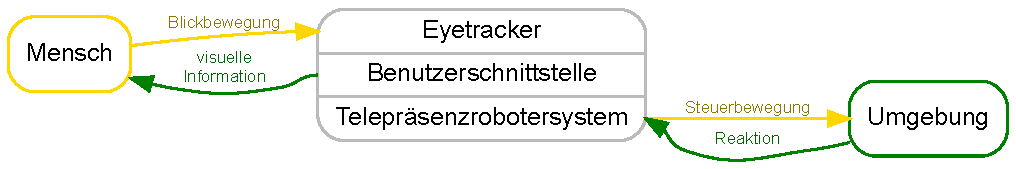
\includegraphics[width=\textwidth]{bilder/grundlagen/simpltrans2.pdf} 
   \end{minipage}% 
\caption{Die Kommunikation zwischen Mensch und Umgebung. Der grundsätzliche Ablauf der Kommunikation ist farblich getrennt hervorgehoben. Mithilfe einer Blickbewegung, die vom Eyetracking-System detektiert wird, kann eine Steuerbewegung des \acl{tps} umgesetzt werden. Die Bewegung kann eine Reaktion der Umgebung erzeugen. Diese Reaktion wird durch das Telepräsenzsystem als Videobild aufgezeichnet und schließlich in Form der visuellen Information über die Benutzerschnittstelle des Systems dem Benutzer zurückgemeldet.}
\label{fig:infotrans}
\end{figure}

Um Strategien zur augenbasierten Steuerung von mobilen Robotersystemen mittels eines Eyetracking-Systems sinnvoll umsetzen zu können, ist es hilfreich, die allgemeine Funktionsweise des menschlichen Auges und seinen Aufbau zu verstehen. Der folgende Abschnitt soll daher zunächst die anatomischen und motorischen Aspekte des Auges darstellen und einführend erklären. Ferner wird auf Erkrankungen mit Bewegungseinschränkungen bei erhaltener Augenbewegung (Okulomotorik) eingegangen und damit eine mögliche Anwendergruppe eingegrenzt. Anschließend werden die in \acs{abb}~\ref{fig:infotrans} skizzierten technischen Komponenten beschrieben. 

\section{Biologische Grundlagen}
\label{section:informationstransfer}
Wie bereits eingangs erwähnt, stellen die Augen bei vielen gravierenden Erkrankungen mit motorischen Beeinträchtigungen oftmals den letzten Kommunikationskanal zur Außenwelt dar. In diesen Situationen kommen ihnen neben rein sensorischen Aufgaben eines Sinnesorgans auch motorische Aufgaben als ausführendes Organ zu. Die Augen nehmen somit eine Art Sonderstellung unter den Sinnesorganen ein und können durch Interpretation der Blickbewegungen zum einen als Indikator für das innere Befinden, das Interesse und die Wünsche eines Menschen dienen und zum anderen als visuelles Eingabesystem für eine grafische Benutzeroberfläche fungieren, ähnlich wie die klassische Computermaus es durch manuelle Eingaben ermöglicht. 

%Um die Blickbewegungen des Benutzers und damit Strategien zur augenbasierte Steuerung von mobilen Robotersystemen zu finden ist es notwendig mit den biologischen Eigenschaften der Augen vertraut zu sein. Der folgende Abschnitt soll daher die anatomischen und motorischen Aspekte des Auges darstellen und einführend erklären.

\subsection{Topografie und Anatomie des Auges}
\label{subsect:topgraf}
Das Auge befindet sich anatomisch in der Augenhöhle (Orbita) des menschlichen Schädels (Cranium) und wird durch mehrere angrenzende Knochenstrukturen stabilisiert und in dieser Position nach dorsal (rückenseits gelegen), medial (zur Mitte hin gelegen) und lateral (zur Seite hin gelegen) geschützt und in seinem Bewegungsumfang begrenzt. Neben dem Augapfel (Bulbus oculi) gehören der Sehnerv (Nervus opticus), die Augenlider, der Tränenapparat und die insgesamt sechs außerhalb des Augenbulbus (extraokulär) angeordneten Augenmuskeln topografisch zum Auge an sich~\cite{Krahn2011}. \acl{abb}~\ref{fig:zugrichtung} zeigt die beschriebenen Strukturen des linken Auges in einer Darstellung von oben. Die Begrenzung des Bulbus nach ventral (bauchseits gelegen) wird vom Ober- und Unterlied (Palpebra superior und inferior) gebildet, in \acs{abb}~\ref{fig:zugrichtung} nicht abgebildet \cite{Krahn2011}. 

\begin{figure}[ht]
   \begin{minipage}[b]{.5\linewidth}          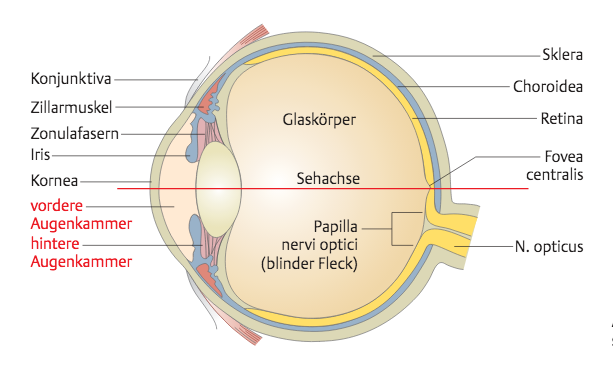
\includegraphics[width=1.05\textwidth]{bilder/grundlagen/g3.png}
      \subcaption{Augapfel (Bulbus oculi)}\label{fig:querschnitt} 
   \end{minipage}% 
   \hfill
   \begin{minipage}[b]{.5\linewidth} 
 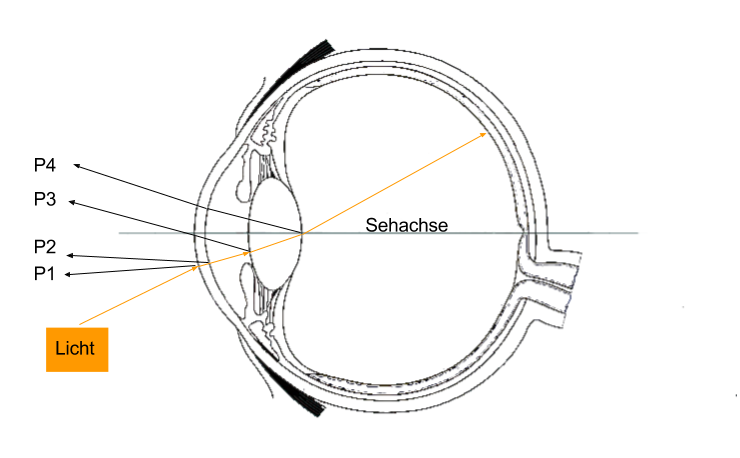
\includegraphics[width=1.05\textwidth]{bilder/grundlagen/g1.png} 
      \subcaption{Purkinje Bilder (P1-P4) }\label{fig:purk}
   \end{minipage}%
   \caption{Das Auges im Längsschnitt mit Darstellung der Anantomie und Lichtreflexion. \textbf{\subref{fig:querschnitt}}~Darstellung der wichtigsten Strukturen des Auges mit den lichtbrechenden Medien; Hornhaut (Cornea), vordere Augenkammer, Linse (Lens cristallina), Glaskörper (Corpus vitreum). \textbf{\subref{fig:purk}}~Entstehung der Lichtreflexionen (Purkinje Bilder) des Auges. Die unterschiedlichen Reflexionen werden nummeriert und mit P1, P2, P3 und P4 bezeichnet. Die Reflexionen resultieren aus der unterschiedlichen Brechkraft der einzelnen Grenzstrukturen im Auge (Vorder- und Rückseite der Cornea, Vorder- und Rückseite der Linse).
(Bild: \textbf{\subref{fig:querschnitt}}~aus \cite[S.438]{Krahn2011},  \textbf{\subref{fig:purk}}~angelehnt an \cite{Krahn2011})}\label{fig:anaauge} 
\end{figure} 

Bei der Betrachtung eines Objektes passiert dessen reflektiertes Licht (elektromagnetische Strahlung mit einer Wellenlänge zwischen 400 und 750 nm) die lichtbrechenden Medien des Auges, siehe \acs{abb}~\ref{fig:anaauge} \cite{Bondke2014}. Jede Struktur hat dabei eine unterschiedliche Brechkraft, die einen Einfluss auf die Gesamtbrechkraft des Auges nimmt. Zu den lichtbrechenden Strukturen zählen somit: (1)~Hornhaut (Cornea), (2)~vordere Augenkammer, (3)~Linse (Lens cristallina) und (4)~Glaskörper (Corpus vitreum).

Die Linse besitzt aufgrund der kollagenhaltigen Zusammensetzung eine Elastizität, die eine Veränderung der Brechkraft ermöglicht, auch bedingt durch den Kontraktionszustand, der innerhalb des Augapfels (intraokulär) gelegenen Muskulatur. Die intraokuläre Muskulatur ist im Rahmen der Nah- und Fernakkommodation aktiv, ferner kann der Lichteinfall durch die Kontraktion und Dilatation der Iris justiert werden. Sobald das Licht die lichtbrechenden Strukturen passiert hat, erscheint das betrachtete Objekt als ein auf dem Kopf stehendes Abbild auf der Netzhaut (Retina) und kann fokussiert werden. Innerhalb der Retina wird die elektromagnetische Strahlung durch lichtempfindliche Rezeptoren (Stäbchen und Zapfen) über ein chemisches Signal in ein elektrisches Signal transferiert und über den Sehnnerv (Nervus opticus, den \RM{2}~Hirnnerv) und die visuelle Nervenbahn in den Hinterhauptslappen des Gehirns (okzipitaler Cortex) geleitet und dort weiterverarbeitet. Durch die Weiterverarbeitung des visuellen Signals entsteht schließlich die visuelle Wahrnehmung und damit die Wahrnehmung der subjektiven Realität des Betrachters. 

\begin{figure}[!ht]
   \begin{minipage}[t]{.5\linewidth} 
      \centering 
      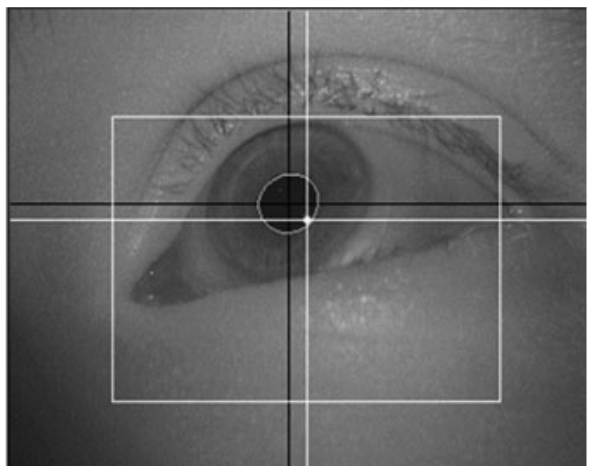
\includegraphics[width=0.94\textwidth]{bilder/grundlagen/Augenreflex.png}
  \subcaption{Corenalreflex des Auges. }\label{fig:purkinje} 
   \end{minipage}% 
   \hfill
   \begin{minipage}[t]{.5\linewidth} 
      \centering 
  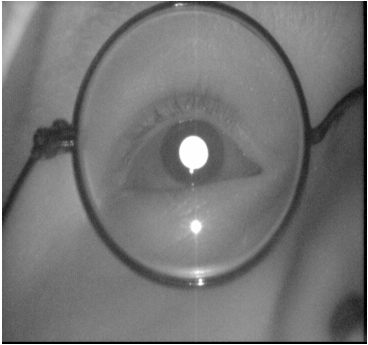
\includegraphics[width=0.8\textwidth]{bilder/grundlagen/reflex.png} 
      \subcaption{Reflexion der Retina.}\label{fig:reflex}
   \end{minipage}%
    \hfill
  \caption{Darstellung ausgewählter Lichtreflexionen des Auges. \textbf{\subref{fig:purkinje}}~Detektion des Corneareflexes und des Pupillenzentrums zur Bestimmung des \acl{por}. \textbf{\subref{fig:reflex}}~Reflexion der Retina. Die Lichtquelle strahlt koaxial zur optischen Achse des Auges, wobei die Netzhaut einen Großteil des Lichtes reflektiert. Dieser Effekt entspricht dem in der Fotografie bekannten Rote-Augen-Effekt. (Bild: \textbf{\subref{fig:purkinje}} aus \cite{Majaranta2014}, \textbf{\subref{fig:reflex}} aus \cite[Abb. 3]{Joos2003})}\label{fig:reflexpurkije} 
\end{figure} 

Bei diesem eben geschilderten Verlauf der Lichtstrahlung wird ein Teil des Lichtes an den beschriebenen lichtbrechenden Strukturen reflektiert und am Auge sichtbar, \vgl \acs{abb}~\ref{fig:purk} und \acs{abb}~\ref{fig:reflexpurkije}. Diese Reflektionen werden als \textit{Purkinje-Bilder} bezeichnet und aufgrund der unterschiedlich reflektierenden Strukturen unterschieden. Das erste Purkinje-Bild entsteht durch die Reflektion an der Außenseite der Cornea (P1), das zweite (P2) durch die Reflexion an der Innenseite der Cornea und das dritte (P3) an der Vorderfläche der Linse. (P4) wird schließlich durch die Grenzfläche an der Rückseite der Linse erzeugt. \acl{abb}~\ref{fig:purk} veranschaulicht das eben Beschriebene. Ein weiteres Phänomen ist die Reflexion der Retina bei einer koaxialen Beleuchtung in Bezug zur optischen Achse des Auges. Siehe \acs{abb}~\ref{fig:reflex} \cite{Joos2003,Eidam2015}. Sowohl die Purkinje-Bilder als auch die Cornealreflektion werden durch Eyetracking-Systeme verwendet, siehe Abschnitt~\ref{section:eyeMet}. 



\subsection{Okulomotorik des Auges}
\label{subsection:okumot}
Die extraokulär angeordnete Muskulatur ist für die Augenbewegungen (Okulomotorik) verantwortlich, siehe \acs{abb}~\ref{fig:zugrichtung}. Grundsätzlich lassen sich durch die Anordnung der extraokulären Muskulatur, die in \acs{abb}~\ref{fig:augenbewegung} dargestellten, drei aufeinander senkrecht stehenden Bewegungsachsen unterscheiden. Der Schnittpunkt dieser Achsen bildet das Drehzentrum des Auges, wodurch folgende willkürliche Bewegungen entlang der genannten Achsen ausgeführt werden können ~\cite{Thoemke2008,Bondke2014}. 

\begin{enumerate}
\item  Abduktions-/Adduktionsbewegungen entlang der vertikalen Achse, die durch den M. rectus medialis und M. rectus lateralis erfolgen, \vgl \acs{abb}~\ref{fig:zugrichtung}. Werden Ab\-duktions- und Ad\-duktionsbewegungen alternierend ausgeführt, entsteht hieraus eine horizontale Augenbewegung. 
\item Elevations-/Depressionsbewegungen entlang der horizontalen Achse, die durch den M. rectus superior und den M. rectus inferior erfolgen,  \vgl \acs{abb}~\ref{fig:zugrichtung}. Werden Elevations,- und Depressionsbewegungen alternierend ausgeführt, entsteht hieraus eine vertikale Augenbewegung.
\item Ex-/Intorsionsbewegungen, also Außen-/Innenrotationsbewegungen entlang der optischen Achse, die durch den M. obliquus superior und M. obliquus inferior erfolgen, \vgl \acs{abb}~\ref{fig:zugrichtung}. Alternierende Bewegungen beider Muskeln in Kombination mit dem \og M. rectus superior und dem M. rectus inferior führen zu diagonalen Augen- oder zu Rotationsbewegungen im Rahmen von Kopfschiefhaltungen.
\end{enumerate}

\begin{figure}[ht]
   \begin{minipage}[t]{.5\linewidth} 
      \centering 
    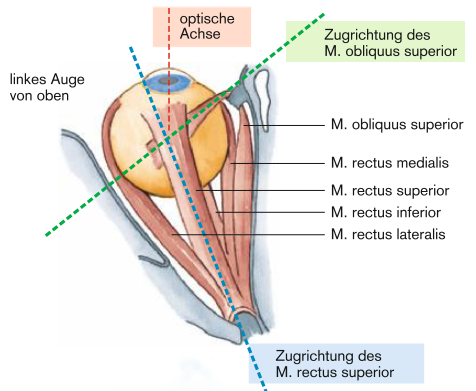
\includegraphics[width=1\textwidth]{bilder/grundlagen/g5.png}
  \subcaption{Linkes Auge von oben}\label{fig:zugrichtung} 
   \end{minipage}% 
   \hfill
 	\begin{minipage}[t]{.5\linewidth} 
      \centering 
   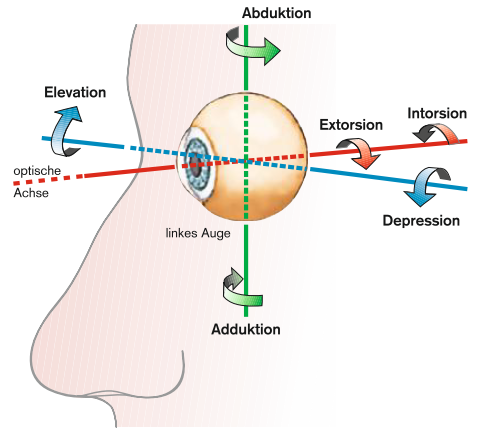
\includegraphics[width=0.9\textwidth]{bilder/grundlagen/g4.png} 
  \subcaption{3 Bewegungsachsen der Augen }\label{fig:augenbewegung} 
   \end{minipage}%
   \caption{Zugrichtung der Augenmuskulatur und Bewegungsachsen. \textbf{\subref{fig:zugrichtung}}~Periokuläre Augenmuskulatur mit fünf der sechs Augenmuskeln. Farblich hervorgehoben ist die Zugrichtung des M. obliquus superior (grün) und des M. rectus superior (blau).  \textbf{\subref{fig:augenbewegung}}~Die drei Bewegungsachsen der Augen mit farblicher Unterscheidung der Abduktions-/Adduktionsbewegungen (grün), Elevations-/Depressionsbewegungen (blau), Ex-/Intorsionsbewegungen (rot). (Bild: aus \textbf{\subref{fig:zugrichtung}}~\cite[S.777]{Bondke2014}, \textbf{\subref{fig:augenbewegung}}~\cite[S.776]{Bondke2014})}\label{fig:augbilder} 
\end{figure} 

Die genannten Bewegungen können willkürlich ausgeführt werden und dienen teilweise als Augengesten im Rahmen der Interaktion mit der implementierten Benutzerschnittstelle.
Eine weitere Bewegung, die für die aktuelle Arbeit von Bedeutung ist, ist die des Lidapparates (Ober- und Unterlied). Der Lidschluss erfolgt durch den in \acs{abb}~\ref{fig:augbilder} nicht dargestellten M. orbicularis oculi~\cite{Krahn2011}. Die Lidöffnung durch den M. levator palpebrae superior, ebenfalls in \acs{abb}~\ref{fig:augbilder} nicht mit abgebildet~\cite{Krahn2011}.

Neben der muskulären Anordnung ist für die Durchführung einer Augenbewegung die nervale Innervation entscheidend. Die sechs Augenmuskeln werden von insgesamt drei Hirnnerven versorgt, die ihren Ursprung in den jeweiligen Hirnnervenkernen im Hirnstamm haben. Somit ist die Ausführung einer regelrechten Augenbewegung maßgeblich von einem intakten Hirnstamm abhängig. Die Versorgung des für die Abduktion zuständigen Augenmuskeln M. rectus lateralis erfolgt über den \RM{6}~Hirnnerv (Nervus abducens). Verletzungen des Muskels oder der nervalen Innervation führen zu einer Störung der Bewegung im Rahmen der horizontalen Augenbewegung. Die Außenrotation (Extorsion) wird über den \RM{4}~Hirnnerv (N. trochlearis) vermittelt und beeinträchtigt die diagonale Blickbewegungen. Darüber hinaus führt die Schädigung des Muskels oder der nervalen Strukturen zu einer Kopfschieflage, um damit die resultierenden Doppelbildern zu kompensieren. Die restlichen Muskeln (M. rectus superior, inferior, medialis; M. obliquus inferior) werden vom \RM{3}~Hirnnerv (N. oculomotorius) innerviert \cite{Bondke2014}. Die Motorik des Lidapparates wird für die Lidöffung vom \RM{3}~Hirnnerv (N. oculomotorius) vermittelt, der Lidschluss durch den N. facialis (\RM{7}~Hirnnerv)~\cite{Krahn2011}.

Zusätzlich zu diesen \og Bewegungen der Augenbuli lassen sich noch Bewegungsformen der visuellen Orientierung und Wahrnehmung unterscheiden~\cite{Bondke2014}, die im Bereich der Detektion von Augengesten von Bedeutung sind. Ziel dieser Blickbewegungen im Rahmen der visuellen Wahrnehmung ist es, den Ort des schärfsten Sehens (Fovea centralis) immer wieder durch schnelle Augenbewegungen auf ausgewählte Fixationspunkte auszurichten, um diese Punkte dadurch zu fokussieren~\cite{Bondke2014}. Die Augenmuskulatur zeichnet sich durch kleine motorische Einheiten (Neuron und Muskelfasern) mit ca. 5 - 10 Muskelfasern pro Motoneuron~\cite{Bondke2014} aus. Im Vergleich zu großen Muskelgruppen im Bereich der unteren oder oberen Extremitäten mit 100 - 1000 Muskelfasern pro Motoneuron. Erst dadurch werden feine und schnelle Bewegungen der Augen ermöglicht. Folgende Bewegungen werde unterschieden und sind aus~\cite{Bondke2014,Thoemke2008,Joos2003} zusammengetragen:

\begin{description}
\item[Fixation] Bezeichnet die Bewegung, die das Fixationsobjekt auf den Ort des schärfsten Sehens abbildet. Während der Fixation finden zur Stabilisierung des Bildes Mikrobewegungen statt. Als Beispiel dient \acs{abb}~\ref{fig:sakkad}.
\item[Sakkaden] Während eines Blickwechsels von einem Objekt zum anderen werden die Augen durch schnelle Augenbewegungen, die sogenannten Sakkaden, zum nächsten Fixationsziel bewegt. Sakkaden gehören zu den schnellsten Muskelbewegungen, die Menschen ausführen können (Winkelgeschwindigkeit bis $ 700 \,^\circ/s $) \cite{Bondke2014}. Für genauere Ausführungen zur Beziehung zwischen Sakkadenamplitude und Sakkadengeschwindigkeit sei auf \cite[S.12 ff.]{Thoemke2008} verwiesen. Zur Verdeutlichung von Sakkaden dient auch hier \acs{abb}~\ref{fig:sakkad}.
\item[Folgebewegung] Befindet sich das fixierte Objekt in Bewegung, werden langsame Bewegungen ausgeführt, um trotz der relativen Bewegung des Objektes eine scharfe und präzise Abbildung auf der Fovea zu erzeugen. Diese Bewegungen erreichen Winkelgeschwindigkeiten bis zu $100 \,^\circ/s$ \cite[S.30]{Thoemke2008}.
\item[Mikrobewegungen] Hierzu zählen Drift, Tremor und Mikrosakkaden, die, wie oben genannt, während der Fixation auftreten. Zum Drift kommt es aufgrund der physiologischen Eigenschaften der Nervenzellen in der Retina, die primär auf Veränderung ausgelegt sind und zur Aufrechterhaltung der Stimulation minimal verändert werden. Diese Driftbewegung wird durch Mikrosakkaden ausgeglichen. Der Tremor wird durch Ungenauigkeiten in der Muskelsteuerung hervorgerufen.
\item[Vergenzbewegungen] Darunter versteht man Ausgleichsbewegungen, die das Auftreten von Doppelbildern bei sich nähernden oder entfernenden Zielobjekten vermeiden. 
\end{description}

\subsection{Erkrankungen mit erhaltener Okulomotorik}
\label{subsect:erkrank}
Im Rahmen der vorliegenden Arbeit soll die Okulomotorik zur visuellen Mensch-Computer-Interaktion i. S. einer Steuerung eines mobilen Robotersystems genutzt werden. Anwendungsgruppen sind Personen mit Sprach- und Bewegungseinschränkungen. Wie bereits im Abschnitt~\ref{subsection:okumot} beschrieben, sind die nervalen Strukturen im Hirnstamm sowie die muskulären Effektoren am Auge entscheidend für eine adäquate Augenkoordination und somit für einen problemlosen Informationstransfer zwischen Mensch und Computer. Dieser Abschnitt benennt mögliche Krankheitsbilder mit erhaltener Okulomotorik bei subtotaler oder totaler Bewegungseinschränkung.

%%%%%%%%%%%%%%%%%%%%%%%%%%%%%%%%%%%%%%%%%%%%%%%%%%%%%%%%%%%%%%%%%%%%%%%%%%%%
%-VENI-VENI-VENI-VENI-VENI-VENI-VENI-VENI-VENI-VENI-VENI-VENI-VENI-VENI-VENI
%-VENI-VENI-VENI-VENI-VENI-VENI-VENI-VENI-VENI-VENI-VENI-VENI-VENI-VENI-VENI

\begin{description}
\item[ALS] Die \acs{als} ist eine Motoneuron-Erkrankung, die mit dem Verlust der motorischen Bewegungen einhergehen kann und bislang nicht heilbar ist. Die Augenkerne im Hirnstamm werden in aller Regel erst spät im Krankheitsverlauf beeinträchtigt, sodass diese als Kommunikationskanal genutzt werden können. Im Spätstadium ist jedoch auch ein kognitiver Abbau bekannt und eine erhöhte Komplikationsrate,- beispielsweise durch eine Atemersatztherapie.
\item[Hoher Querschnitt (traumatisch, demyelinisierend, entzündlich, neoplastisch)] Ein hoher Quer\-schnitt kann traumatisch bedingt, also durch Verletzungen der Halswirbelsäule auf Höhe der Halswirbelkörper C3-C5 verursacht werden, welcher mit einer Muskelschwäche bis hin zur Muskellähmung aller vier Extremitäten (Tetraparese oder Tetraplegie) und damit verbundener Immobilität einhergehen kann~\cite{VanMiddendorp2014a}. Des Weiteren kann ein hoher Querschnitt durch demyelinisierende Erkrankungen (\zB Multiple Sklerose), neoplastische Raumforderung (spinale Tumoren) oder durch Entzündungen (Hirnstammencephalitis, Abszess) mit Veränderungen des Rückenmarkes auf cervikaler Ebene hervorgerufen werden.
\item[Hypoxischer Hirnschaden] Dies ist eine Schädigung des Gehirns, die durch verschiedenen Erkrankungen/Unfälle infolge von Sauerstoffminderversorgung des Gehirns entstanden ist. Diese Form kann sich verschieden klinisch manifestieren und ist abhängig von der Schädigungslokalisation im Gehirn. 
\item[Schlaganfälle] (Ischämie oder Blutung): Ein Schlaganfall entsteht zum Großteil entweder durch eine Gefäßthrombose und damit einhergehende Sauerstoffminderversorgung der betroffenen Gehirnareale oder durch eine Blutung und damit verbundenem Zelluntergang und Schädigung des Gehirns. 
\item[\acf{lis}] Das \acs{lis} wird durch eine bilaterale Schädigung der ventralen Pons (Brücke) des Hirnstamms verursacht, die zu einer Tetraplegie und Anarthrie (Ausfall der Sprechfunktion) bei erhaltenem Bewusstsein führt~\cite{Khanna201196}. Ursachen können zum einen Durchblutungsstörungen der Arteria basilaris, die für die Blutversorgung des Hirnstamms zuständig ist, sein, zum anderen Blutungen und Entzündungen des Hirnstamms. Für ein~\acs{lis} können ebenso Tumore im Hirnstamms oder eine pontine Myelinolyse ursächlich sein, welche durch zu rasche Korrektur des initial erniedrigten Blutnatriumspiegels zu einer Schädigung der Pons führt~\cite{steven2005}. Nach Bauer et al. (1979)~\cite{Bauer1979} wird das \acs{lis} durch den Grad der motorischer Beeinträchtigung unterteilt in (a)~\textit{klassisches LIS}, das dadurch charakterisiert wird, dass eine komplette Immobilität vorherrscht, jedoch sowohl die vertikale Augenbewegung als auch die Augenlidbewegung möglich ist. (b)~\textit{inkomplettes LIS} erlaubt willkürliche Bewegungen und (c)~\textit{totales LIS} beinhaltet die komplette Immobilität auch der Augenbewegungen bei erhaltener Bewusstseinslage~\cite{Khanna201196}.
\end{description}

Nachfolgend wird als nächste Komponente im Rahmen einer Kommunikation zwischen Mensch und Umwelt auf Eyetracking-Systeme eingegangen.

\section{Eyetracking-Systeme}
\label{section:eyetracker}

Nach der ausführlichen Beschreibung der Okulomotorik und der anatomischen Eigenschaften der Augen soll der folgende Abschnitt das technische Hilfsmittel zur Detektion und Nutzung von Blick- und Augenbewegungen den Eyetracker einleitend vorstellen. Dabei wird ein Überblick über die Eyetracking-Methoden gegeben. Ferner wird der spezielle Nutzen von Eyetracking-Systemen als Eingabegerät zur Steuerung einer Benutzerschnittstelle beschrieben. Dieses Kapitel orientiert sich inhaltlich an den Ausführungen von Majaranta und Bulling (2014), sowie an Lupu (2013) und Hollomon et al. (2017)~\cite{Lupu2013,Majaranta2014,Hollomon2017}. 

\subsection{Eyetracking-Methoden}
\label{section:eyeMet}
Eyetracking-Systeme haben sich initial aus dem Wunsch der Menschen entwickelt, Einblicke in die Physiologie der Augenbewegung zu erhalten, um den visuellen Apparat als Sinnesorgan genauer zu verstehen. Die Entwicklung von Methoden zur Aufzeichnung von Augenbewegungen gehen auf das Jahr 1879 zurück, als Emile Java, ein französischer Augenarzt, Selbstversuche während des Lesens mithilfe eines einfachen Spiegels aufzeichnete~\cite{Lupu2013}. Eyetracking-Systeme haben sich seitdem durch den technischen Fortschritt weiterentwickelt und befinden sich seit mehreren Jahrzehnten, beispielsweise in der psychologischen und neurowissenschaftlichen Forschung, als diagnostisches Werkzeug zur Erforschung kognitiver Prozesse und Intentionen der Benutzer im Einsatz~\cite{Duchowski2002}.

Allgemein bezeichnet Eyetracking eine Methode, die es ermöglicht, die Augenbewegungen eines Anwenders zu erfassen und daraus auf seinen aktuellen Betrachtungspunkt zu schließen. Der Betrachtungspunkt wird auch als sogenannter \acf{por} bezeichnet. Damit können die genaue Blickbewegung und -position des Anwenders während der Nutzung in Relation zu unterschiedlich präsentierten Stimuli untersucht werden~\cite{SMI2011}. \acl{abb}~\ref{fig:sakkad} zeigt die durch ein Eyetracking-System aufgezeichneten und farblich hervorgerufenen Blickpositionen beim Lesen eines Textes. Die Darstellung veranschaulicht die bereits in Abschnitt~\ref{subsection:okumot} charakterisierten Augenbewegungen, die durch die Nutzung eines Eyetracking-Systems sichtbar werden. 
 
\begin{figure}[ht]
   \begin{minipage}[b]{\linewidth} 
      \centering 
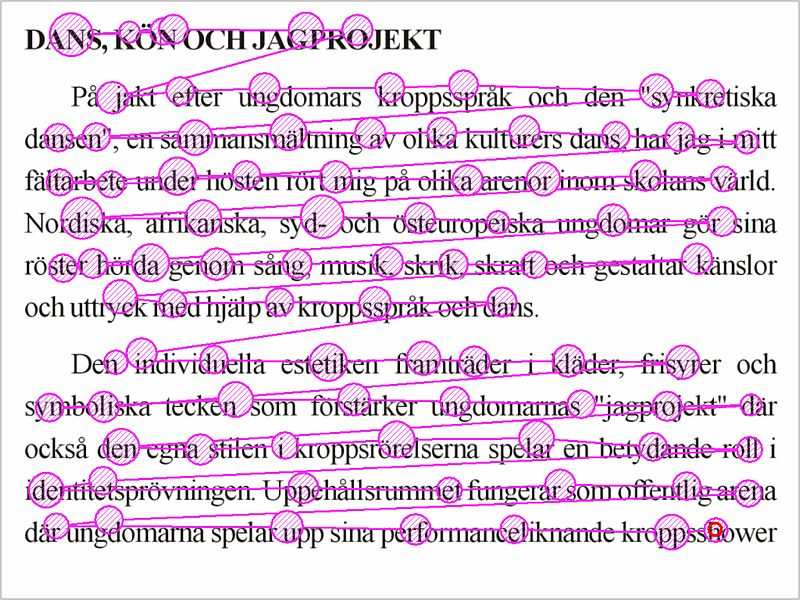
\includegraphics[scale=3]{bilder/grundlagen/sakkaden.jpg}
   \end{minipage}% 
   \hfill
   \caption{Fixation und Sakkaden während des Lesens (schwedischer Text). Aufzeichnung eines videobasierten Eyetracking-Systems der Firma \acs{smi} während eines Schnelllese-Wettbewerbs. Zu Erkennen, sind die als runde Punkte dargestellte Fixierungen, getrennt durch schnellen Sakkadenbewegung. (Bild: aus \url{https://commons.wikimedia.org/wiki/File:Reading_Fixations_Saccades.jpg} letzter Aufruf: 6. Februar 2017)}\label{fig:sakkad} 
\end{figure}

Die Methodik der Detektion hat sich initial von invasiven Verfahren hin zu aktuell weitgehend noninvasiven Techniken weiterentwickelt~\cite{Joos2003,Lupu2013}. Nachfolgend werden einige ausgewählte Verfahren beschrieben, die zur Detektion von Augenbewegungen verwendet werden.  Für weitere Methoden sei auf Joos et al. (2003) und Young und Sheena (1975) verwiesen~\cite{Joos2003, Young1975}.

\begin{description}
\item[Elektrookulografie] Dieses Verfahren mittels \acs{eog} macht sich die natürliche elektrische Potenzialdifferenz zwischen der Vorder- und Hinterseite des Augenbulbus zur Detektion der Augenbewegung zunutze, \vgl \acs{abb}~\ref{fig:pmsub1}. Die Potenzialdifferenz entsteht durch einen negativen Pol am Augenfundus und einem positiven Pol an der Hornhaut~\cite{Lupu2013,Barea2002}. Dabei ist die Potenzialdifferenz mit einer Spannung von 0.4 bis 1.0 mV ausreichend, um diese mittels fünf periorikulär angebrachten Elektroden zu messen, siehe \acs{abb}~\ref{fig:pmsub2} \cite{Lupu2013}. Erfolgt eine gerichtete Augenbewegung, entsteht durch die Richtung der Bewegung ein unterschiedlicher Spannungsverlauf zwischen den angebrachten Elektroden. Für eine genauere Ausführung sei auf \cite{Joos2003} verwiesen. Die Detektion der Augenbewegung beruht auf dem Verhältnis zwischen Blickwinkel~$\sigma$ und der Spannung~$U$, wobei die Spannungsdifferenz bis zu einem Blickwinkel von $40\,^\circ$ annähernd proportional ist: $U_0 = U_0 * sin \sigma$ \cite{Joos2003}. 

\begin{figure}[ht]
   \begin{minipage}[b]{0.5\linewidth} 
      \centering 
  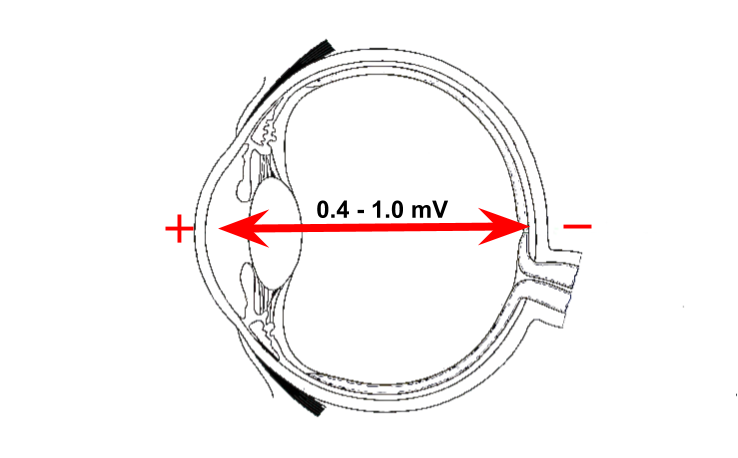
\includegraphics[width=1\textwidth]{bilder/grundlagen/plusminus.png}
    \subcaption{Potenzialdifferenz des Auges}\label{fig:pmsub1}
   \end{minipage}% 
   \hfill
   \begin{minipage}[b]{0.5\linewidth} 
      \centering 
  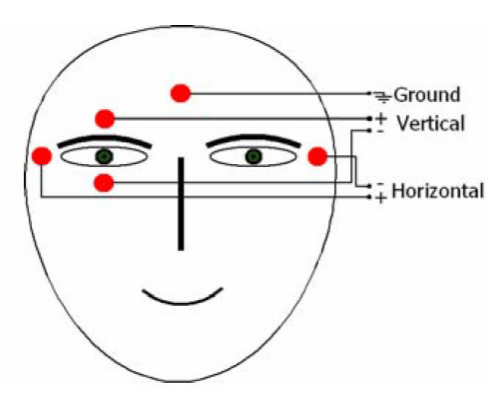
\includegraphics[width=0.8\textwidth]{bilder/grundlagen/eog.png}
  \subcaption{periokuläre Elektroden}\label{fig:pmsub2}
   \end{minipage}% 
   \hfill
   \caption{\acf{eog} mit der Positionierung der Elektronen. (Bild: \subref{fig:pmsub1}und \subref{fig:pmsub2} angepasst aus \cite[S.74]{Lupu2013})}\label{fig:plusminus} 
\end{figure} 

\item[\enquote{Bright Pupil}-Verfahren] Es basiert auf einem Algorithmus, der sich die Reflexion der Cornea, also das Purkinje-Bild (P1) und das Pupillenzentrum zur Bestimmung des \acs{por} zunutze macht. Als Lichtquelle wird ein Infrarotlicht verwendet, wodurch der Benutzer im Vergleich zum sichtbaren Licht nicht geblendet wird. Durch die Positionierung der Lichtquelle eng an der optischen Achse des Auges erfolgt eine Lichtreflexion durch die Netzhaut. Die Pupille erscheint hell (bright) und lässt sich mittels einer zum System gehörenden Kamera aufzeichnen. Aus dem Videobild werden unter Zuhilfenahme von Bilderkennungsalgorithmen das Pupillenzentrum und der Cornealreflex detektiert. Der resultierende Vektor der beiden Punkte, der sich in Abhängigkeit der Blickposition verändert, lässt letztlich auf den \acs{por} des Benutzers schließen \cite{Poole2005}. \acl{abb}~\ref{fig:schemaPurk} verdeutlicht diese Beschreibung und zeigt die helle Pupille und den Cornealreflex schematisch aus Sicht der Kamera. Der Cornealreflex verändert sich in Relation zum Pupillenzentrum in Abhänigkeit der Blickposition.
\item[\enquote{Dark Pupil}-Verfahren] Diese Methode basiert,- auf denselben Prinzipien wie das Bright-Pupil-Verfahren. Die Pupille wird jedoch in einem anderen Winkel beleuchtet und erscheint aus diesem Grund dunkel (dark). Das Bright-Pupil-Verfahren und das Dark-Pupil-Verfahren zählen zur Gruppe der videobasierten Eyetracking-Methoden. Die vorliegende Arbeit basiert auf dem letzterem Prinzip.

\begin{figure}[ht]
\begin{minipage}[t]{\linewidth} 
      \centering 
      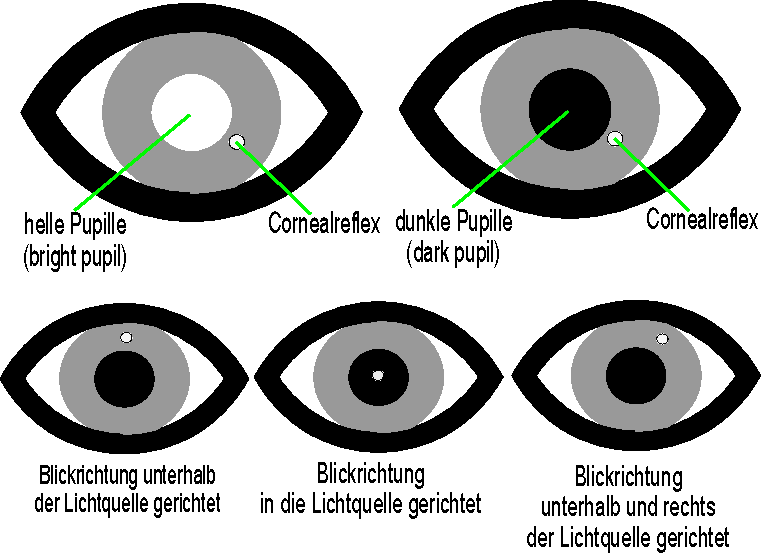
\includegraphics[scale=0.7]{bilder/grundlagen/eye22.pdf}
  \caption{Schematische Darstellung eines Auges mit unterschiedlicher Abbildung Bright- \bzw Dark-pupil Verfahrens (oben). Veränderung des Cornealreflexes in Abhängigkeit der Blickbewegung (unten). (Darstellung angelehnt an Pool et al.~\cite{Poole2005}).}\label{fig:schemaPurk} 
   \end{minipage}% 
\end{figure}
\end{description}

Eyetracking-Systeme ermöglichen neben der Erfassung des \acs{por} die Bestimmung weiterer Parameter,- wie \zB die Erfassung des Pupillendurchmessers, des Lidschlusses, der Anzahl der Fixationen an einem bestimmten Punkt, oder der Dauer der Fixationen an unterschiedlichen Punkten \cite{Joos2003,Jacob2003, Poole2005}. Ferner lassen Parameter wie der sogenannte Scan-Path, also die Folge des Fixationsverlaufs oder der Bereich des Blickfeldes, der besonders häufig beobachtet wird (Area of interest), Rückschlüsse auf das Interesse des Nutzers \cite{Jacob2003,Lupu2013, Peters2013} zu. Für die vorliegende Arbeit stehen die Erfassung der Blickbewegung \bzw der Fixation, der horizontalen und vertikalen Augengeste und die Erkennung des Lidschlusses im Vordergrund.

Nachfolgend werden einige Eigenschaften des für die vorliegende Arbeit verwendeten videobasierten Eyetracking-Systems beschrieben.

\subsection{Eigenschaften videobasierter Eyetracking-Systeme}
\label{section:vidMet}
Videobasierte Eyetracking-Systeme werden heutzutage unter den verwendeten Eyetracking-Systemen häufig verwendet \cite{Poole2005,SMI2011}. Vorteile dieser Systeme liegen in der wenig invasiven Technik und der robusten Augen\-detektion \cite{SMI2011}. 
Diese Systeme lassen sich zusätzlich zur Detektionsmethode durch den Befestigungsort des \textit{\aclp{et}~(ETM)} unterscheiden. Damit ist die Komponente gemeint, die meistens sowohl die Infrarot-Lichtquelle,- als auch die aufzeichnende Kamera enthält. Bei mobilen \textit{\acl{hed}} Systemen ist die Kamera an einem Brillengestell oder einer Helmvorrichtung angebracht, siehe \acs{abb}~\ref{fig:eyeTrackingsub1}. Auf eine Positionierung des Eyetrackingmoduls am Kopf des Anwenders verzichten \textit{stationäre Eyetracking-Systeme}, siehe \acs{abb}~\ref{fig:eyeTrackingsub2}.

\begin{figure}[ht]
   \begin{minipage}[t]{0.5\linewidth} 
      \centering 
      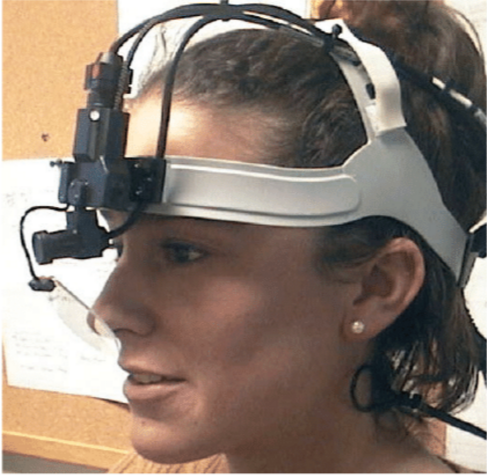
\includegraphics[width=.7\textwidth]{bilder/grundlagen/HDM.png}
     \subcaption{\acl{hed}}\label{fig:eyeTrackingsub1}
   \end{minipage}% 
   \hfill
   \begin{minipage}[t]{0.5\linewidth} 
      \centering 
      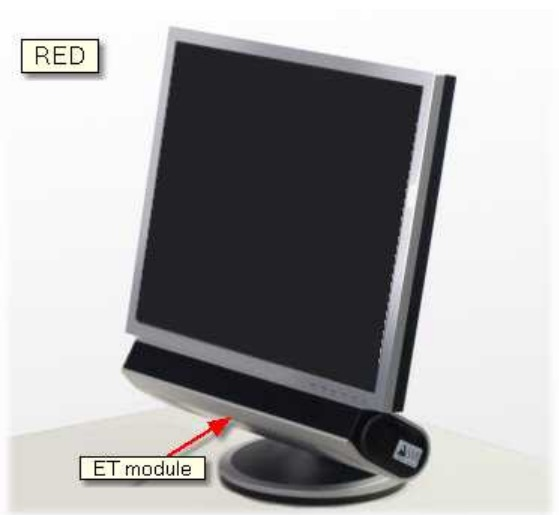
\includegraphics[width=0.8\textwidth]{bilder/implementierung/Eye3.JPG}
   \subcaption{stationäre Eyetracker }\label{fig:eyeTrackingsub2}
   \end{minipage}% 
    \hfill
   \caption{Darstellung zweier videobasierter Eyetracking-Systeme. (Bild: \textbf{\subref{fig:eyeTrackingsub1}}~\cite{Goldberg2003}, \textbf{\subref{fig:eyeTrackingsub2}}~\cite[S.136]{SMI2011})}\label{fig:device} 
\end{figure} 

Die vorliegende Arbeit verwendete das stationäre System \acf{red} der Firma \acf{smi}, das in \acs{abb}~\ref{fig:eyeTrackingsub2} dargestellt ist. \acl{abb}~\ref{fig:eyeTrackingsub2} zeigt die typische Positionierung des \acs{et} mit Kamera und Infrarot- Lichtquelle unter oder neben dem stimuluspräsentierenden Monitor. Die Position lässt sich jedoch auch variieren.  Das in \acs{abb}~\ref{fig:eyeTrackingsub2} gezeigte \acs{et} ist aufgrund zweier Infrarot-Lichtquellen auch für eine binokularen Nutzung ausgelegt \cite{Eidam2015,SMI2011}. Damit ist prinzipiell eine getrennte Detektion der Augenbewegungen der Augenpaare möglich. Standardmäßig gehört gewöhnlich auch eine Computereinheit, die die oben erwähnten bildverarbeitende Algorithmen zur Berechnung des \acs{por} ausführt, zu den Komponenten eines videobasierten Systems. 

Bei stationären Systemen wie dem \acs{red}-System ist eine bestimmte Positionierung der Versuchsperson und der Augenposition zur Optimierung des Detektionsergebnisses wichtig. Die schematische Darstellung des Herstellers in \acs{abb}~\ref{fig:empfehlung} verdeutlicht die empfohlene Anordnung. Er empfiehlt bei der Durchführung eine Entfernung von 60 - 80 cm vom \acs{et} einzuhalten.

\begin{figure}[ht]
\begin{center}
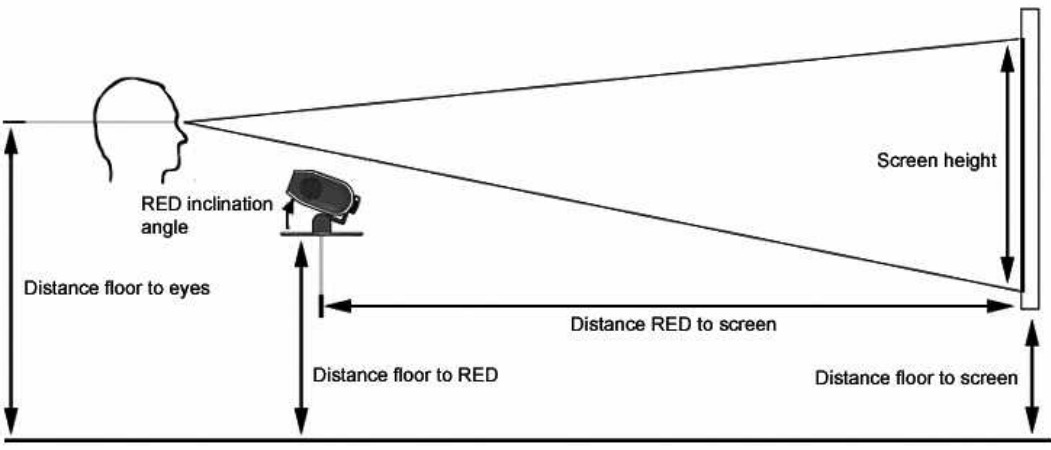
\includegraphics[width=0.7\textwidth]{bilder/grundlagen/Schema.JPG}
\end{center}
\caption{Schema der empfohlenen Anordnung.
Die Positionierung des \acs{et} im Verhältnis zur Kopfposition. (Bild: aus \cite[S.150]{SMI2011})}
\label{fig:empfehlung}
\end{figure}

Ferner ist zur präzisen Berechnung des \acs{por} eine Kalibrierung für videobasierte Eyetracking-Systeme individuell für jeden Anwender im Vorfeld der Nutzung notwendig. Dabei ist auch eine Instruktion des Anwenders vor Beginn der Benutzung sinnvoll. Bei der Kalibrierung werden definierte Punkte am Bildschirm angezeigt, während vom System die entsprechenden Pupillenpositionen in Abhängigkeit der Bildschirmkoordinaten erfasst und intern zur Optimierung des \acs{por} verwendet werden.  

Weitere Faktoren, die die Qualität der Detektion der Augenposition reduzieren können, sind neben der Kopf- \bzw Augenpositionierung,- schlechte Lichtverhältnisse, Brillengläser, tief hängende Augenlieder oder auch Make-up. Ferner können durch Kopfbewegungen Fehlinterpretationen seitens des Systems entstehen, auch wenn diese intern teilweise kompensiert werden können \cite{SMI2011}.

Nach den eben beschriebenen Eigenschaften und dem Aufbau videobasierter Eyetracking-Systeme, sowie der Methodik zur Detektion von Augengesten ist im Weiteren die damit verbundene Interaktion mit einer grafischen Benutzerschnittstelle relevant. 

\subsection{Augengesten als Eingabemechanismus für grafische Benutzer\-ober\-flächen}
\label{subsection:eingabemech}

Die Anwendungsmöglichkeiten eines Eyetracking-Systems reichen von der Funktion als passive Informationsquelle, beispielsweise in der Forschung, bis hin zu einem aktiven Eingabemechanismus,- \zB während der Bedienung einer grafischen Benutzeroberfläche \cite{majaranta2011,Majaranta2014}. Während einerseits die Augenbewegungen eher im Hintergrund aufgezeichnet werden und damit keine speziellen Anforderungen an den Benutzer gestellt werden, finden andererseits willkürlich kontrollierte Augenbewegungen als Steuersignale für ein Computersystem Anwendung und somit werden Anforderungen an die kognitiven Fähigkeiten des Benutzer gestellt \cite{majaranta2011,Majaranta2014}. 

Trotz dieser Anforderungen bieten Eyetracking-Systeme als Eingabemedium zur Interaktion mit einer grafischen Benutzeroberfläche Einsatzmöglichkeiten speziell für Menschen mit motorischen Beeinträchtigungen \cite{Majaranta2014,Eidam2015,Eidam2016}. 

Der in der vorliegende Arbeit verwendete Prototyp dient ausschließlich als Eingabegerät zur Interaktion mit einer grafischen Benutzeroberfläche und nutzt explizit definierte Augengesten als aktive Steuersignale zur Bedienung eines mobilen Robotersystems. 

Um mit Elementen einer grafischen Benutzeroberfläche wie \zB mit Knöpfen (Buttons) und mit kleinen Symbolgrafiken (Icons) zu interagieren, müssen vom Eingabegerät hauptsächlich Zeige- und Selektionsoptionen bereitgestellt werden. Die Computermaus als klassisches manuelles Eingabegerät erfüllt diese Funktion durch die Repräsentation der eigenen relativen Position als eine abstrakte Zeiger- \bzw Fingerposition auf dem Bildschirm \cite{Peters2013}. Der Benutzer kann durch Positionierung des Mauszeigers auf Elemente der grafischen Benutzerschnittstelle einfache Zeigehandlungen ausführen. Durch das Betätigen der Maustasten (klicken) kann ein Element gezielt selektiert werden. Mit einer Computermaus sind darüber hinaus noch \textit{Drag-And-Drop}- Operationen möglich \cite{Peters2013}; also die Interaktion mit ausgewählten Elementen der Benutzeroberfläche in Form eines Verschiebens und Loslassens dieser Elemente.

Um mithilfe eines Eyetracking-Systems zumindest Zeige- und Selektionsoperationen realisieren zu können, sind die in Abschnitt~\ref{subsection:okumot} genannten Augenbewegungen relevant, die als Steuerkommandos verwendet werden können. In der Literatur wurden unterschiedliche Blick- und Augengesten im Hinblick auf ihre Nützlichkeit und Effizienz als Eingabesignal untersucht, \vgl~\cite{Hollomon2017,Eidam2015,Poole2005}. Folgende Auflistung zeigt mögliche Augenbewegungen als Eingabesignal und die damit verbundenen Eigenschaften. 

\begin{description}
\item[Blickbewegungen] Durch die motorischen Eigenschaften der Augen besteht die Möglichkeit, Blickbewegungen, also den \acs{por} als Eingabesignal für die Bewegung eines Cursors am Bildschirm, zu verwenden. Damit lassen sich Zeigehandlungen am Bildschirm, wie sie auch mit der Computermaus möglich sind, durchführen. Blickbewegungen ermöglichen ein natürliches und schnelles Zeigen. Dies liegt zum einen daran, dass Menschen ihren Blick häufig aktiv auf Gegenstände oder Objekte richten, die für den Beobachter eine gewisse Relevanz haben, und zum anderen daran, dass, noch bevor sie eine andere aktive Handlung durchführen können, das Objekt erblickt haben \cite{majaranta2011}. Die Augen sind somit früher bei einem potenziell relevanten Objekt angelangt, als es durch den Einsatz einer Computermaus möglich wäre. 

Für Selektionsaufgaben in grafischen Benutzerschnittstellen eignet sich die Blickbewegung jedoch nur unter gewissen Umständen. Grund hierfür ist das sogenannte Midas-Touch-Problem. Darunter versteht man die Fehlinterpretation einer Augengeste als Interaktionsabsicht, während der Benutzer nur um sich blicken wollte und keine Steuerintention verfolgte \cite{Majaranta2014,majaranta2011}. Im Unterschied zu einer Computermaus kann beispielsweise der \acs{por} als Cursorzeiger nicht einfach an einer Stelle des Bildschirms belassen werden, während andere Bereiche des Bildschirms inspiziert werden. Eine einfache Inspektion der Benutzeroberfläche ist dadurch nicht mehr möglich, da jeder Blick als Interaktionsabsicht interpretiert wird. Somit kann die Blickbewegung als Eingabesignal nur unter bestimmten Bedingungen als Selektionssignal für eine klassische Benutzerschnittstelle verwendet werden. Bei einer großen Anzahl von Interaktionselementen wie Icons und Buttons eignet sich diese Geste nur sehr bedingt. Besteht eine grafische Benutzeroberfläche jedoch aus wenigen, gut sichtbaren Elementen, kann die Selektion per Blickgeste die Interaktion vereinfachen, da dadurch unbeabsichtigte Interaktion und damit das Midas-Touch-Problem weit weniger prominent ist. Für die vorliegende Arbeit wurde die Blickgeste als Steuersignal durch eine begrenzte Anzahl der Elemente der Benutzeroberfläche verwendet. Für genauere Ausführungen sei auf Abschnitt~\ref{chapter:implementierung} verwiesen.
\item[Fixation mit unterschiedlicher Verweildauer] Die Eigenschaften, die bereits für die Blickbewegung beschrieben wurden, gelten analog auch für die Fixation. Im Grunde handelt es sich bei der Blickbewegung um eine Fixation mit nur sehr kurzer Verweildauer. Es bietet sich jedoch an, durch variable Verweildauern,- das \og Midas-Touch-Problem zu reduzieren. So kann beispielsweise ein Element der grafischen Benutzeroberfläche bei längeren Verweildauern eine gewisse Zeit betrachtet werden, ohne gleich ein Selektionssignal zu erzeugen. Dadurch wird dem Benutzer ermöglicht, Elemente genauer zu inspizieren, je nach Dauer der Fixierung. Verlängert man diese Zeitperiode jedoch weiter, kann dies im Falle einer Selektionsabsicht schnell zu langsamen und unnatürlichen Verhalten während der Interaktion führen. Für verkürzte Zeitperioden gilt das für die Blickbewegung bereits Beschriebene. Die Zeitdauer stellt somit eine Methode dar, zwischen einer Zeige- und einer Selektionsabsicht zu unterscheiden. In der Literatur haben sich für natürlich empfundene Interaktionen Zeiten im Bereich von 150-300 ms etabliert \cite{Hollomon2017,Eidam2015,majaranta2011}. Zeiten größer 750 ms werden als störend und unnatürlich empfunden \cite{Hollomon2017}. 
\item[Blinzeln und Zwinkern] Auch der Lidschluss mit beiden Augen, also das Blinzeln - oder nur mit einem Auge das Zwinkern - wurde als Augengeste in Abschnitt~\ref{subsection:okumot} beschrieben und kann als Eingabesignal für eine Interaktion mit einer Benutzerschnittstelle verwendet werden. Häufig wird diese Augengeste jedoch nicht einzeln zu Selektionszwecken verwendet, sondern in Kombination mit Blick-oder Fixationsgesten. Probleme können dabei allerdings zum einen durch die Missinterpretation des natürlichen Blinzeln im Rahmen der Benetzung der Cornea mit Tränenflüssigkeit entstehen, zum anderen stellt das Zwinkern eine eher unnatürliche Geste dar, die nach gewisser Zeit zu Ermüdungen führen kann \cite{Hollomon2017}. Ferner ist das Zwinkern bei Menschen mit motorischen Beeinträchtigungen häufig aufgrund von nur einem funktionsfähigen Auge nicht sinnvoll umzusetzen. Um natürliches von bewusstem Blinzeln als Steuersignal zu unterscheiden, sind ähnlich wie bei der Fixation bestimmte Zeitkriterien relevant. Hier lassen sich Zeiten von 150 ms bis 250 ms als in der Literatur sinnvoll beschriebene Zeitdauer festlegen \cite{Eidam2015}. Nach Eidam und Hollomon et al. liegt in einer Kombination von Blick- \bzw Fixationsgesten und der Lidschlussgeste eine effiziente Eingabemethode vor \cite{Hollomon2017,Eidam2015}.
\item[Horizontale, vertikale Augenbewegungen] Um eventuell weitere Operationen durch die Augengesten bereitzustellen, können sowohl horizontale als auch vertikale Augenbewegungen verwendet werden. Aus der Vorgängerarbeit von Eidam ließen sich jedoch speziell für die horizontale Augengeste Probleme während der Ausführungen feststellen, da diese Augenbewegungen in ihrer reinen Ausführung eher unnatürlich sind \cite{Eidam2015}. Horizontale Augengesten spielen jedoch nur eine untergeordnete Rolle, da Personen mit Bewegungseinschränkung bei noch erhaltener Augenmotorik häufig nur vertikale Augenbewegungen ausführen können \cite{Eidam2015}.  
\item[Pupillendilation] Sie wird in dieser Aufzählung nur der Vollständigkeit halber aufgeführt. Zwar gibt es Versuche, die Pupillendilation zur Steuerung von Spielen zu verwenden \cite{Ekman2008}, allerdings sind hier intensive Vorbereitungen notwendig, die nicht von jeder Person durchgeführt werden können. Im Rahmen der vorliegenden Arbeit spielen sie aus diesem Grund keine Rolle bei der Interaktion mit der Benutzeroberfläche.
\end{description}

Wie die Auflistung der möglichen visuellen Steuersignale gezeigt hat, stellt die blick- und augenbasierte Interaktion mit einer Benutzeroberfläche eine Herausforderung dar. Dies resultiert zum einen aus der bereits in Abschnitt~\ref{subsection:okumot} erwähnten Doppelfunktion des Auges als Sinnesorgan und als Effektororgan, zum anderen aus der Problematik, die potenziell mehrdeutigen Augenbewegungen aufseiten des Systems den richtigen Steuerintentionen des Benutzers zuzuordnen \cite{majaranta2011, Majaranta2014, Hyrskykari2006}. Trotzdem zeigt die Auflistung, dass eine Interaktion durch eine geeignete Kombination der Augenbewegung und sinnvolle Konzeption der grafischen Benutzerschnittstelle an die Bedürfnisse einer visuellen Steuerung durchaus sinnvoll eingesetzt werden kann. 


\section{Telepräsenzrobotersysteme}
\label{section:tps}
Robotersysteme spielen in der Medizin und der Gesundheitsversorgung seit einigen Jahrzehnten eine immer wichtigere Rolle \cite{tsui2011,Tsui2014,Tonin2011,Michaud2010,Labonte2010}. Der folgende Abschnitt beschreibt zunächst die Begriffe \textit{Telepräsenz} und \textit{Teleoperation}. Im Anschluss folgt eine Beschreibung des allgemeinen Aufbaus von \acs{tps} und der möglichen Anwendungsgebiete dieser Systeme. Abschließend wird auf die speziellen Anforderung für eine Steuerung aus der Ferne eingegangen. 

\subsection{Teleoperation und Telepräsenz}
\label{section:tele}
Bevor auf die Komponenten eines Telepräsenzrobotersystems genauer eingegangen wird, sollen zunächst die Begriffe \textit{Telepräsenz} und \textit{Teleoperation} erörtert werden. 

Die ersten grundlegenden Konzepte der Telepräsenz gehen auf den amerikanischen Kameramann und Erfinder Morton Heilig (22.12.1926–14.05.1997) zurück \cite{Peters2013}. Seine aus den 1950er- Jahren stammenden Ideen, eine möglichst realitätsgetreue Kinowahrnehmung durch das Einbeziehen aller Sinne nachzubilden, war der damaligen Zeit deutlich voraus \cite{packer2002,Peters2013}. Erzeugt werden sollte ein Gefühl des \textit{sich in der Umgebung Befindens\footnote{im Sinne von \textit{an einem Ort präsent sein}.}} \cite{Peters2013}. 

Auch für Marvin Minsky (09.08.1927-24.01.2016) lag in der Entwicklung von Telepräsenzsystemen ein beträchtlicher Reiz \cite{Minsky1980}. So stellte er sich vor, dass Menschen mit Sensoren ausgestattete Kleidung benutzen, um damit entfernte Robotersysteme beispielsweise für Arbeitstätigkeiten zu steuern. Die gemessenen Bewegungen der Kleidungssensoren, sollten eins zu eins in motorische Bewegungen des entfernten Roboters umgesetzt werden. Minsky ging sogar so weit, dass auch das Gefühl beispielsweise eine entfernte Roboterhand zu benutzen, nicht von der Benutzung der eigenen Hand zu unterscheiden sein sollte \cite{Minsky1980}. 

Ein derartiges Gefühl der Telepräsenz wurde nach all den Jahren auch heute technisch in der vorgeschlagen Form noch nicht erreicht. Nichtsdestotrotz hat die Entwicklung von \acl{tps} in den letzten Jahren Fortschritte gemacht, wie die Beispiele in \acs{abb}~\ref{fig:bilder} exemplarisch veranschaulichen. Diese kommerziell erhältlichen Systeme können als ein verkörpertes Videokonferenzsystem auf Rädern beschrieben werden \cite{Tsui2011b}. Sie erzeugen eine physische Anwesenheit mit flexibler Mobilität,- zusätzlich zu den Kommunikationsmöglichkeiten, die durch das Videokonferenzsystem gegeben sind \cite{Tsui2011b}.

Eng verbunden mit dem Begriff der Telepräsenz ist der aus dem Gebiet der Telerobotik stammende Begriff der \textit{Teleoperation}. Sie bezeichnet die Ausführung (\textit{operation}) einer Aktion durch ein entferntes (\textit{tele}) Robotersystem \cite{Rossler2009}. Dabei erfolgt die Steuerung durch eine visuelle Rückmeldung des mobilen Systems, \zB über einen Bildschirm, auf dem das Videobild der entfernten Umgebung zu sehen ist. Der Nutzer kann das System durch die visuelle Rückmeldung beispielsweise mit einem Joystick aus der Entfernung steuern.  Allgemein muss aufseiten der steuernden Person der Zustand des Robotersystems und der Umgebung möglichst gut bekannt sein. Man bezeichnet dies als \textit{situation~awareness~(SA)}~\cite{Drury2003,Yanco2004-2}. Die Effizienz der Steuerung hängt entscheidend von der \acs{sa} ab \cite{Drury2003,Yanco2004-2}. Weitere Ausführungen folgen in Abschnitt~\ref{section:steuerung}

Wie oben beschrieben, geht die Telepräsenz im Vergleich zur Teleoperation, über die reine Ausführung einer Operation hinaus und zielt auf ein Eintauchen in die Umgebung mit allen Sinnen und Wahrnehmungen ab \cite{Rossler2009}. Damit liefert die Teleoperation einen -wenn man so will- geringeren Grad der Immersion \cite{Rossler2009}. Dieder Grad der Immersion hängt jedoch von beeinflussbaren Faktoren wie \zB der Qualität der Bilddarstellung und der Konsistenz der wahrgenommenen Eindrucke ab \cite{Rossler2009,Peters2013}.

All diese beschriebenen Eigenschaften eines Telepräsenzrobotersystems erscheinen speziell für Personen mit eingeschränktem Bewegungsradius, beispielsweise aufgrund des Alters, aufgrund von körperlichen Bewegungseinschränkungen oder anderer Ursachen, umso bedeutender, da sich in dieser Konzeption ein telepräsentes mobiles Robotersystem dazu eignet, den Bewegungsumfang zu erweitern. Ferner ermöglicht es die Herstellung von sozialen Interaktionen zwischen Individuen auch über eine große Entfernung hinweg \cite{Kristoffersson2013,sheridan1992,Tsui2014}. 

Das nachfolgende Kapitel beschreibt die Komponenten, die einen Einfluss auf die erlebte Immersion des Systems haben und zu einem \acs{tps} gehören.

\subsection{Komponenten eines Telepräsenzrobotersystems}
\label{subsection:komponenten}

Aktuell erhältliche kommerzielle \acs{tps} unterscheiden sich in vielen Aspekten wie Größe, Beweglichkeit und Anwendungsfeld (\vgl~\acs{abb}~\ref{fig:bilder}). Es gibt jedoch auch Eigenschaften, die unter den verschiedenen Systemen konstant und vergleichbar sind. Desai et al. charakterisiert mehrere Aspekte, die für \acs{tps} essenziell sind \cite{Desai2011}:

\begin{description}
\item[Video] Die Videoinformation ist eine entscheidende Komponente für die Interaktions- und Navigationsmöglichkeit des \acs{tps}. Yanco und Drury (2004) zeigten, dass sich Benutzer bei der Nutzung von \acs{tps} am stärksten auf die Videoinformationen mehr als auf andere Informationsquellen verließen \cite{Yanco2004}. Aufgrund der Beweglichkeit der mobilen Roboter müssen die Videodaten kabellos transferiert werden. Dies erhöht das Augenmerk auf die Netzwerkverbindung. Hierbei ist ein Trade-off zwischen den unterschiedlichen Charakteristika der Netzwerkverbindung zu legen. Die Blickfeldgröße, die Farbschärfen und die Auflösungen haben Einfluss auf die Verbindung. Eine geringe Bildqualität kann im Rahmen der Navigation Schwierigkeiten verursachen. Ferner kann eine bessere Bildqualität die Latenz der Verbindung erhöhen. All diese Aspekte sollten bei der Konzeption und für den individuellen Anwendungsrahmen bedacht werden.
\item[Audio] Für die Kommunikation über ein \acs{tps} sind die Aspekte der Audioinformation relevant. Hierbei sind die Audioqualität sowie die adäquate Lautstärke wichtige Einflussgrößen. Die verschiedenen Umgebungslautstärken können eine Adjustierung der Lautstärke verlangen.
\item[\acf{ui}] Die Benutzerschnittstelle des Systems ist als Komponente für die Steuerung des \acs{tps} von Bedeutung, da sich der Benutzer und der mobile Roboter an unterschiedlichen Lokalisationen befinden und die Benutzerschnittstelle die Verbindung zu beiden Lokalitäten bereitstellt. Das Wissen über die Umgebung des \acs{tps}, über seine Aktivität und seinen Zustand wird ausschließlich über die Benutzerschnittstelle präsentiert. So kann es abhängig vom Anwendungsgebiet des \acs{tps} fundamental wichtig sein, den exakten Systemzustand zu kennen. Benutzerschnittstellen für entfernte mobile Robotersysteme können nach Yanco et al. in zwei Kategorien eingeteilt werden: video- oder karten-zentrierte Benutzerschnittstellen \cite{Yanco2007,Keyes2010}.
Die Benutzerschnittstelle sollte in ihrer Konzeption leicht in der Handhabung und nicht einschränkend bezüglich der Bereitstellung von Informationen sein, gleichzeitig jedoch durch eine zu große Fülle an Informationen wenig überfordern \cite{Desai2011}. 
\item[Physische Eigenschaften] Eigenschaften wie die Größe und das Gewicht eines \acs{tps} sind wichtige physische Eigenschaften des Systems. So können Robotersysteme, die klein und wendig sind, in Bereichen eingesetzt werden, die für große Robotersysteme unerreichbar sind. Gleichzeitig ist die Stabilität größerer Systeme in anderen Bereichen vorteilhaft. Die Größe ist auch entscheidend in Bezug auf die Positionierung der Kamera und dem dadurch erzeugten Blickwinkel und -bereich. Häufig kann eine Ansicht, die eine Übersicht der Umgebung liefert, für die Routenplanungen zweckmäßiger sein. Hingegen sind für das gezielte Ansteuern von Gegenständen die Höhen der Gegenstände relevanter. Einige \acs{tps} bieten häufig zwei oder mehrere Kamerasysteme an, die die Vorteile beider Systeme vereinigen \cite{Kristoffersson2013}. 
Auch die Geschwindigkeit des \acs{tps} und ihre flexible Anpassung während der Fahrt ist eine Komponente mit vielen Vorteilen.
\item[Autonome Navigation] Autonome Navigation kann für sicherheitsrelevante Aufgabenstellungen des Systems unerlässlich sein. Die Benutzung und Steuerung eines mobilen Robotersystems erfordert gewisse kognitive Fähigkeiten des Benutzers. Die Konzentrationsfähigkeit, die Merkfähigkeit und die räumliche Orientierung sind für den vermehrten kognitiven Aufwand mitverantwortlich. Assistive Steuerungssysteme können diesen kognitiven Mehraufwand in Bezug auf \enquote{niedrigere} Steuerungsaufgaben wie beispielsweise das Ausweichen von Hindernissen reduzieren und auf \enquote{höhere} Aufgaben wie beispielsweise Routenplanungsvorhaben oder gezielte Interaktionen legen.  
\item[Soziale Gegebenheiten] Aufgrund der Interaktionsmöglichkeit mit der Umwelt, haben \aclp{tps} neben den oben genanten technischen und funktionalen Eigenschaften auch soziale Aspekte für den Benutzer des Systems. Diese Eigenschaften tragen zu einer Akzeptanz des Systems bei \cite{Goodrich2013}. 
\end{description}

\begin{figure}[ht]
   \begin{minipage}[t]{.25\linewidth} 
      \centering 
    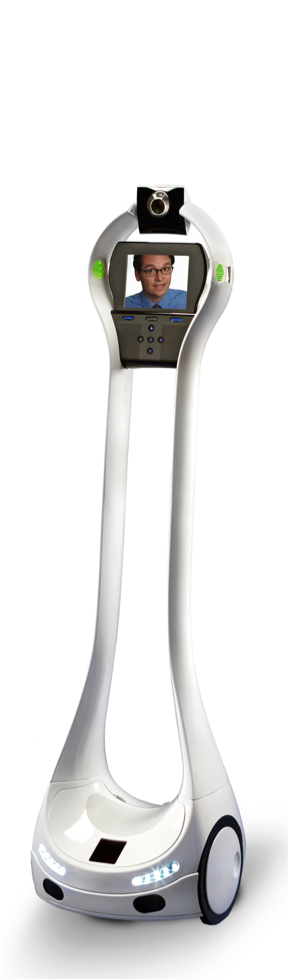
\includegraphics[width=0.66\textwidth]{bilder/grundlagen/1.png} 
      \subcaption{VGo}\label{fig:w} 
   \end{minipage}% 
   \hfill
   \begin{minipage}[t]{.25\linewidth} 
      \centering 
      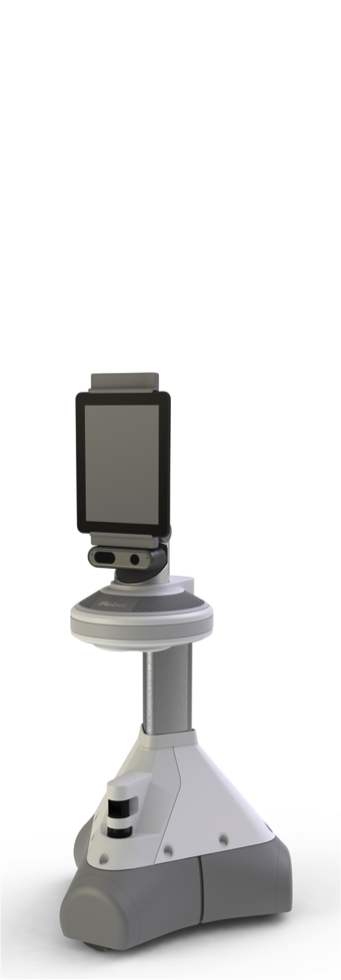
\includegraphics[width=0.78\textwidth]{bilder/grundlagen/2.png} 
      \subcaption{iRobot Ava}\label{fig:x} 
   \end{minipage}%
   \hfill
   \begin{minipage}[t]{.25\linewidth} 
      \centering 
      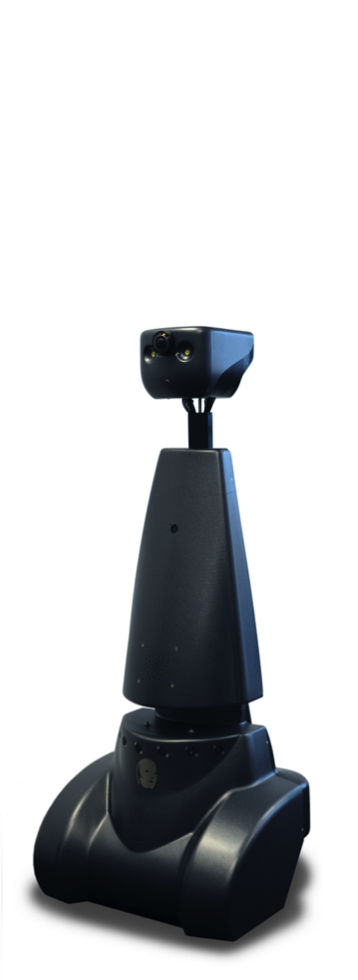
\includegraphics[width=0.8\textwidth]{bilder/grundlagen/3.png}
      \subcaption{Gostai Jazz}\label{fig:y} 
   \end{minipage}%
   \hfill
   \begin{minipage}[t]{.25\linewidth} 
      \centering 
      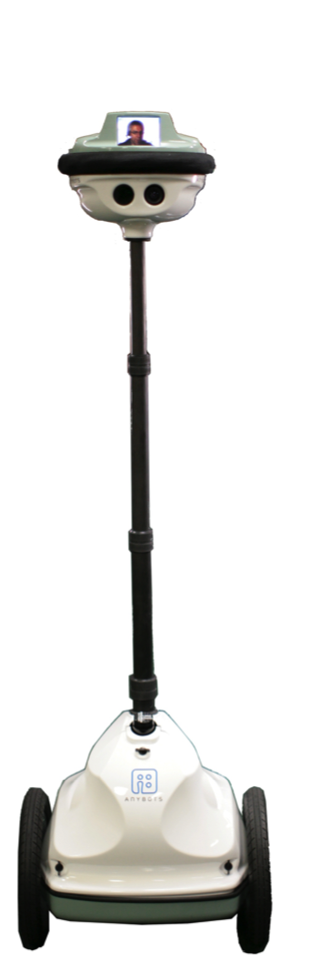
\includegraphics[width=0.7\textwidth]{bilder/grundlagen/4.png} 
      \subcaption{Anybots QB}\label{fig:z} 
   \end{minipage}%
   \hfill
   \caption{Eine Auswahl an \aclp{tps} im Vergleich. Zu Erkennen sind die Komponenten der einzelnen Telepräsenzrobotersysteme wie beispielsweise die Videokomponente, die eine Abbildung der benutzenden Person darstellt, und eine oder mehrere Videokameras, die die Umgebung filmen. Zu erkennen ist auch der unterschiedliche Aufbau der Systeme. (Bilder: aus  \cite{Kristoffersson2013})}\label{fig:bilder} 
\end{figure} 

Der Nutzen der Systeme zeigt sich in unterschiedlichen Anwendungsgebieten. Der folgende Abschnitt orientiert sich vornehmlich an den Ausführungen von \cite{Kristoffersson2013} und beschreibt allgemeine Anwendungsfelder von \acs{tps}.

\subsection{Anwendungsgebiete von Telepräsenzrobotersystemen}
\label{section:anwendungTPS} 

Die im Abschnitt \ref{subsection:komponenten} beschriebenen Eigenschaften und Komponenten der \aclp{tps} können innerhalb einiger Anwendungsfelder sinnvoll angewandt werden. So beschreibt \cite{Kristoffersson2013} Anwendungsgebiete im Bereich der Medizin, Gesundheitsversorgung, aber auch im Umfeld von Bürotätigkeiten und sicherheitsrelevanten Bereichen. Die folgende Aufzählung zeigt einen Überblick über die erwähnten Anwendungsfelder: %Anwendungsszenarien in der Medizin und Gesundheitsbereich werden  Im speziellen wird es um das Anwendungsfeld der Gesundheitsversorgung von Patienten mit Sprach- und Bewegungseinschränkung gehen, da dies im Fokus der Abschlussarbeit steht.

\begin{description}
\item[Unternehmens- und Büroaktivitäten] In global agierenden Unternehmen wird beispielsweise aufgrund der Vernetzung der Mitarbeiter in \ua international kooperierenden Gruppen ein immer größerer Wert auf die Kommunikation gelegt. \acs{tps} können in diesem Umfeld die Kommunikation und Kooperation untereinander sinnvoll ergänzen. Bereits 2002 gab es erfolgreiche Versuche, die Anwendung von mobilen \acs{tps} beispielsweise in  Unternehmenskonferenzen oder Sitzungen zu testen \cite{Jouppi}. Der Wunsch, \acs{tps} in wirtschaftlichen Szenarien zu etablieren, kann einmal in der Zeitersparnis durch das Wegfallen eventueller Reiseaktivitäten als auch in einer unmittelbaren Bereitstellung von Wissen durch geeignete Mitarbeiter in jedem Augenblick gesehen werden \cite{Jouppi}. Auch für Führungskräfte kann die Einflussnahme unter Umständen durch \aclp{tps} erweitert werden.
\item[Sicherheitsrelevante Bereiche] Neben den Anwendungsgebieten in Unternehmen, kann man sich mobile \acs{tps} auch in Bereichen vorstellen, die Sicherheitsrisiken für einen Menschen darstellen. So wurden während der Nuklearkatastrophe in Fukushima 2011 das \acl{tps} \textit{PackBot} der Firma iRobot verwendet, um Erkundungen innerhalb erhöhter Strahlenexpositionsgebiete vorzunehmen\footnote{\url{https://de.wikipedia.org/wiki/Nuklearkatastrophe_von_Fukushima} (letzter Aufruf: 04. März 2017)}.
\item[Gesundheitsversorgung, Medizin] Auf diesem Gebiet gibt es mehrere interessante Anwendungsbeispiele. Stepan Sopin, ein an Leukämie erkrankter Schüler, konnte mit einem \acs{tps} namens \textit{R.BOT 100} während seines Genesungsprozesses am Unterricht teilnehmen\footnote{\url{http://www.newsamen.com/101339/robot-goes-to-school-for-sick-kids-video} (letzter Aufruf: 04. März 2017)}. Auch Fels et al. (2001) beschreibt Anwendungsfelder von \acs{tps} für Schüler und Studenten~\cite{Fels2001}. 


Für die Verwendung von mobilen Robotersystemen im Anwendungsgebiet der Gesundheitsversorgung, beispielsweise bei älteren Personen mit körperlichen Beeinträchtigungen, werden nach Tsui et al. (2011) prinzipiell folgende Szenarien als mögliche Anwendungsfälle unterschieden \cite{tsui2011}. Diese Szenarien können auch auf die für diese Arbeit im Fokus stehende Personengruppe angewandt werden.

\begin{figure}[ht]
   \begin{minipage}[b]{\linewidth} 
      \centering 
      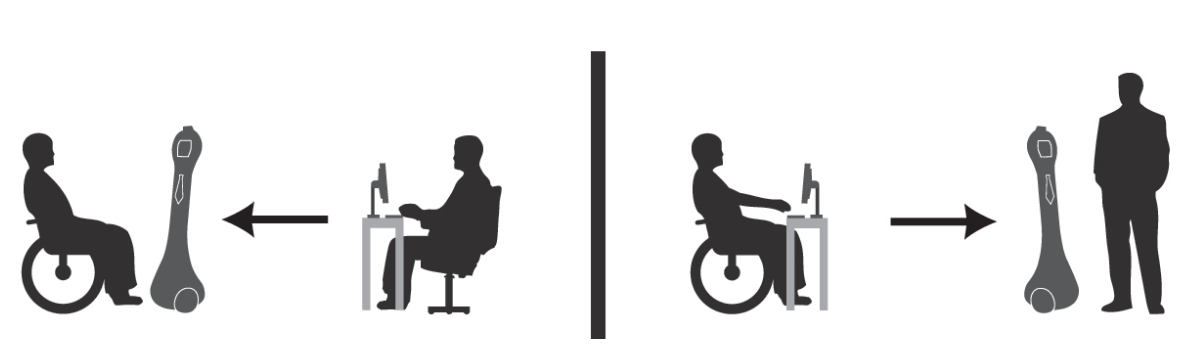
\includegraphics[width=0.7\textwidth]{bilder/grundlagen/Szenario.png}
      %\missingfigure{Darstellung aus Majaranta und Bulling (2014)}
   \end{minipage}% 
   \caption{(Links)~Szenario 1 \acs{tps} von Familienmitglied, Arzt oder Pflegekraft gesteuert, (Rechts)~Szenario 2 \acs{tps} von immobiler Person gesteuert (Bild: aus \cite[S.1]{tsui2011})}\label{fig:szenario} 
\end{figure} 

\begin{description}
\item[Szenarion 1] In diesem Szenario wird das \acs{tps} in die unmittelbare Umgebung der Person mit den körperlichen Beeinträchtigungen positioniert. Die Steuerung des \acs{tps} wird von Angehörigen, Ärzten oder Pflegepersonal übernommen. Dadurch ist es möglich, falls gewünscht, eine fast ununterbrochene Überwachung der hilfebedürftigen Person zu gewährleisten. Dieser Anwendungsfall wurde für Ärzte in Krankenhäusern bereits während der Visiten bei Patienten mit chirurgischen Eingriffen getestet \cite{Ellison2004}. Auch für Familienangehörige kann es sinnvoll sein, auf diese Art und Weise mit dem Familienmitglied zu interagieren.
\item[Szenarion 2] Das zweite Szenario steht im Fokus der vorliegenden Arbeit. Hierbei wird das \acs{tps} von einer Person mit Bewegungseinschränkung verwendet. Es wird in einer Umgebung positioniert, die seitens der Person mit der Bewegungseinschränkung erkundet oder mit der interagiert werden soll. Diese Umgebung kann auch die eigene Wohnung sein, wodurch der eingeschränkte Bewegungsumfang deutlich erweitert werden kann. Kinder, die beispielsweise krankheitsbedingt oder entfernungsbedingt nicht in der Schule anwesend sein können, können trotzdem durch die Unterstützung eines \acs{tps} wieder virtuell an der Klassengemeinschaft teilhaben\footnote{\url{http://www.dallasobserver.com/news/lyndon-baty-and-the-robot-that-saved-him-6429680} (letzter Aufruf: 08. Februar 2017)}. 
\end{description}
Für den Fall, dass das \acs{tps} in der Nähe der hilfebedürftigen Person verbleibt, sind die in Szenario 1 und 2 genannten Möglichkeiten kombinierbar. Ferner kann man sich eine Möglichkeit vorstellen, unterschiedliche Telepräsenzsysteme von einer Person zu kontrollieren, ähnlich wie es von Dr. Roey Tzezana, einem israelischen Wissenschaftler, vorgeschlagen wurde\footnote{\url{https://www.youtube.com/watch?v=zevLw5SbGvM} (letzter Aufruf: 08. Februar 2017)}.

\end{description}

Um \aclp{tps} im Rahmen der \og Anwendungsfelder adäquat nutzen zu können, muss eine gut funktionierende Teleoperation der Systeme gewährleistet sein. Daher geht der folgende Abschnitt auf die Teleoperation von Robotersystemen ein.

\subsection{Teleoperation von Robotersystemen}
\label{section:steuerung}

Eine gut funktionierende Steuerung eines mobilen Robotersystems ist für eine sichere und natürliche Interaktion in und mit der Umgebung (einschließlich der Personen in der Umgebung) eine wichtige Voraussetzung für die Akzeptanz des Systems \cite{Tsui2014}. Die Steuerung muss verlässlich und präzise die Steuerabsichten des Benutzers umsetzen. Hierbei sind neben dem Faktor der Umgebung (\zB~Hindernisse, Menschen und Tiere) auch die Vorerfahrungen der Benutzer im Umgang mit der Teleoperation von mobilen Robotersystemen relevant, wie die Arbeit von Casper und Murphy (2003) im Kontext der Terroranschläge in New York 2011 zeigt \cite{Casper2003,Labonte2010}.
Die visuellen Informationen und die implementierten Steuermethoden, die durch die Benutzerschnittstelle bereitgestellt werden, sind weitere Faktoren, die zu einer besseren situation~awareness und damit zu einer effizienteren Teleoperation von mobilen Robotersystemen beitragen \cite{Scholtz04,Yanco2004-2,Labonte2010,Tsui2014,Goodrich2013}.

%Gängige Systeme sind die haptischen und Grundsätzlich lassen sich hierbei 
Die Interaktion mit Robotersystemen erfolgt heutzutage weitgehend durch haptische Interaktionsmechanismen \cite{Dunser2015}, beispielsweise durch die Computermaus, die Tastatur oder einen Steuerhebel (Joystick). 

%Nach Peters et al. (2013) lassen sich haptische Eingabemechanismen nach aus der Physik bekannten mechanischen Gleichgewichtslagen einteilen, vgl. \cite[S.118]{Peters2013}. Hiernach wird zwischen \textit{stabilen}, \textit{labilen} und \textit{indifferenten} Gleichgewichtslagen unterschieden \cite{Peters2013}. Angewandt auf haptischen Eingabegeräte können sich in der Interaktion zwischen Eingabemechanismus und Benutzer die dynamischen Veränderungen des Mechanismus ebenfalls stabil, labil und indifferent Verhalten. Beispiel für



\begin{comment}
\begin{figure}[ht]
   \begin{minipage}[b]{\linewidth} 
      \centering 
\fbox{\includegraphics[width=\textwidth]{bilder/grundlagen/Kugel.png}}
   \end{minipage}% 
   \hfill
   \caption{}\label{fig:kugel} 
\end{figure}

\end{comment}


%Um eine Steuerung eines Computersystems zu ermöglichen von Heutzutage liegt der Schwerpunkt in Bezug auf die Interaktion mit einem Computersystemen 
 % einen Ein in der Mensch-Computer Interaktion besteht und und  sowohl für die Die Mensch-Computer Interaktion im Kontext der Teleoperation von Robotersystemen, stellt sowohl Anforderungen an das System als auch an den Benutzer selbst.

%Die Teleoperation von Robotersystemen basiert auf speziell entwickelte Benutzerschnittstellen, diese müssen um eine zielgerechte Interaktion über eine Distanz zu ermöglichen den Zustand des Telepräsenzsystems möglichst genau wiedergeben.

%Die Steuerung von Robotersystemen und damit der Informationstransfer von Mensch zu Computer basiert auf unterschiedlichen Eingabesystemen. 
Dabei lassen sich in Abhängigkeit des Einflusses des Benutzers auf die aktive Steuerung unterschiedliche Steuermethoden unterscheiden. Goodrich et al. (2013) unterscheidet folgende \cite{Goodrich2013}.
%Neben einer direkten Steuerung durch den Benutzer des \acs{tps} der dazu führt, dass alle an den mobilen Roboter übertragenen Signale vom Roboter umgesetzt werden lassen sich noch weitere erweiterte Steuermethoden nach G \cite{Goodrich2013}.
\begin{description}
\item[Supervisory control] Hierunter wird eine intermittierende Steuerungsmethode verstanden, wobei eine oder mehrere Benutzer nach jedem Steuerbefehl auf die Rückmeldung des Roboters warten; so kann Schritt für Schritt ein beabsichtigter Weg beschritten werden~\cite{sheridan1992}.
\item[Direct control] Darunter wird die direkte Umsetzung der Steuersignale durch das mobile Robotersystem verstanden. Die von Minsky visionierte Interaktion kann zu dieser Methode gezählt werden, \vgl~Abschnitt~\ref{section:tele}. 
\item[Shared control] Die steuernde Person sendet die beabsichtigten Steuerkommandos an den mobilen Roboter. Im Gegensatz zur direkten Kontrolle während der \textit{direct control}-Methode führt der mobile Roboter weiterhin die Steueranweisungen aus, verändert sie jedoch in Abhängigkeit von  auftauchenden sicherheitsrelevanten oder steuerungsrelaventen Aspekten, \zB beim Ausweichen eines Hindernisses. Dadurch kann sich der Benutzer auf andere Aspekte konzentrieren. Vergleiche dieser Methoden werden in \cite{Baldo2015} gezeigt.
\item[Traded control] Diese Methode erweitert die \textit{shared control}-Methode,- dahingehend, dass der Benutzer das Bewegungsziel vorgibt,- und der Roboter die Aufgaben eigenständig ausführt, bis die Aufgabe oder das Ziel erfüllt wurde.
\end{description}

Nach Abschluss der Beschreibung aller wichtigen Komponenten für die Umsetzung einer blick- und augenbasierten Steuerung eines mobilen Robotersystem mithilfe eines Eyetracking-Systems, wird in dem folgenden Kapitel~\ref{chapter:fragestellung} auf die vorgesehen Lösungsstrategien und die zu untersuchenden Testmerkmale eingegangen. 

%Die Steuerung einer Benutzeroberfläche mittels Blick- oder Augenbewegungen zu gewährleisten, stellt eine Herausforderung dar \cite{Hollomon2017}. Zwar ist die Augenmotorik willkürlich kontrollierbar, dennoch gibt es wie \og viele unwillkürliche Augenbewegung im Rahmen der Wahrnehmung und Orientierung. Es gilt somit, zwischen beabsichtigten Steuersignalen und unbeabsichtigten Blickbewegungen des Benutzers zu unterscheiden. Das Auge, welches primär als Sinnesorgan zur Perzeption der Umwelt dient, übernimmt wie in Abschnitt \ref{subsection:okumot} gezeigt, willkürliche Steueraufgaben durch die extraokuläre Muskulatur. Damit fungieren die Augenmuskulatur als Steuerinstanz, ähnlich wie es die Hand und Fingermuskulatur bei der Eingabe durch die Maus oder Tastatur erfüllen. Die Eingabemöglichkeit hängt mit den möglichen Augenbewegungen zusammen. In der vorliegenden Arbeit werden (Blickbewegungen, Lidschluss, Fixation, vertikaler Augenbewegung) als definierte Augengeste verwendet.



%\item Midas-Touch: Aufgrund der bereits \og Doppelfunktion des Auges als Sinnesorgan im Rahmen der visuellen Wahrnehmung und gleichzeitig als motorisches Effektororgan \zB Im Rahmen von Steueraufgaben kann es zum sogenannten Midas-Touch Problem kommen \cite{Majaranta2014}. Hierunter versteht man die Fehlinterpretation einer Augengeste als Steuersignal, wenn der Benutzer nur umher blickt und keine Steuerintention verfolgt. Im Unterschied zu einer Computermaus kann beispielsweise der \acs{por} als Mauszeiger nicht einfach an einer Stelle des Bildschirms belassen werden, während andere Bereiche des Bildschirms betrachtet werden. Dies ist bei der manuellen Steuerung mit der Computermaus ohne Probleme möglich. Auch das gewohnte \enquote{klicken} bei der Verwendung der Computermaus um \zB Buttons zu selektieren, kann nicht ohne Probleme in der Augensteuerung umgesetzt werden. Die Fixationen als Selektionsmechanismus können zu unabsichtlichen Betätigungen führen. Dies lässt sich zu einem gewissen Grade mittels der Kombination mehrerer Augengesten als Selektionsmechanismus beheben \cite{Majaranta2014}. 


%Grundsätzlich lassen nach Majaranta et al. sich Eyetracking-Systeme

%Majaranta und Bulling (2014) teilen die allgemeinen Nutzungsmöglichkeiten in vier Kategorien ein, siehe Abbildung \ref{fig:continuum}.

\begin{comment}


\begin{figure}[ht]
   \begin{minipage}[b]{\linewidth} 
      \centering 
      \includegraphics[width=1\textwidth]{bilder/grundlagen/D170203.png}
      %\missingfigure{Darstellung aus Majaranta und Bulling (2014)}
   \end{minipage}% 
   \caption{Mögliche Nutzungsmöglichkeiten von Eyetrackingdevices (Bild: \cite[S.52]{Bondke2014}) }\label{fig:continuum} 
\end{figure} 
\end{comment}
%So gibt es blickbasierte- Text Eingabesysteme für Menschen mit Bewegungseinschränkung. Diese Systeme ermöglichen es mittels eines zusätzlichen Kommunikationskanals, die Lebensqualität der Benutzer deutlich zu verbessern und ihr Leben ein Stück aktiver zu gestalten.


%\item Genauigkeit: Der entscheidente Faktor für die Genauigkeit der Eyetrackingmethode sind die 

%\end{itemize}
%In der Literatur werden 5 explizite Blickgesten für die Steuerung untersucht. 
%(a) Fixation mit unterschiedlichen Intervallen, (b) Blinzeln und Zwinkern, (c) 



\begin{comment}

Es ergibt sich hierdurch die Möglichkeit der individuellen Nutzung des Eyetrackings für eine große Bandbreite von Anwendungsgebiete unter anderem für wissenschaftliche Zwecke \cite{SMI2011}.

Im Rahmen dieser Abschlussarbeit werden die  All diese Messparameter sich für unterschiedliche Anwendungsfelder relevant. Für einen Überblick sei auf die Ausführungen von Duchowski (2002) verwiesen \cite{Duchowski2002}.


Es folgt eine   Die Bewegung der Augenbulbi wird auf unterschiedliche Messmethoden . und die Augenbewegungen aufzuzeichnen und hieraus mittels verschiedener Messverfahren den \acf{por} des Benutzers zu berechnen. D Die Bestimmung des \acs{por} durch Eyetracking-Systeme benutzen unterschiedliche unterschiedliche anatomisch-physiologischen Eigenschaften des Auges die Augenbewegungen.   



Die Bestimmung der Blickposition wird durch ein Messverfahren ermöglicht welches auf der Distanz zwischen dem Mittelpunkt der Pupille und dem \og ersten Purkinjebild, welches durch die Reflektion einer Lichtquelle an der Vorderseite der Hornhaut entsteht. Dieser Messvorgang läuft völlig kontaktlos ab und benötigt lediglich eine adäuate Positionierung der Benutzenden Person vor der Lichtquelle.  Durch diese Möglichkeiten kommt das Eye-Tracking als technisches Hilfsmittel in vielen Anwendungsgebiete zu Einsatz. 

\subsection{Augenbasierte Interaktion}
Manuelle Eingabegeräte wie beispielsweise die Computermaus
Augenbewegungen als Steuersignale für ein Eingabegerät zu verwenden bietet sicherlich Nachteile 

%Für Marvin Minsky (09.08.1927 - 24.01.2016) lag in der Entwicklung von Telepräsenzrobotersystemen eine beträchtliche Innovationsmöglichkeit, von welcher er bereits in den achtziger Jahren überzeugt war \cite{Minsky1980}. So stellte er sich beispielsweise vor, Menschen mit Sensoren ausgestattete Kleidung benutzen zu lassen um damit entfernte Robotersysteme zu steuern, welche die gemessenen Bewegungen der Kleidungssensoren, eins zu eins in motorische Bewegungen des Roboters umsetzen können. Minsky ging sogar soweit, dass auch das Gefühl beispielsweise eine entfernte Roboterhand zu benutzen nicht von der Benutzung der eigenen Hand zu unterscheiden war. Damit habe man das Gefühl sich in der entfernten Umgebung anwesend zu fühlen, obwohl man sich dort nicht aufhält. 

%Die Wahrnehmung oder das Gefühl sich in einer anderen Umgebung als der aktuellen, präsent oder anwesend zu fühlen, bezeichnet Kristoffersson et al. als \textit{Telepräsenz} \cite{Kristoffersson2013}. Ein mobiles \acf{tps} ermöglicht es einem Benutzer, der dieses System steuert und durch die Komponenten des \acs{tps} einen Einblick in die entfernte Umgebung erhält, sich derartig mit dieser Umgebung zu verbinden, dass er sich in der entfernten Umgebung frei und unbeeinträchtigt von ortsbedingten Gegebenheiten der eigenen Umgebung bewegen kann \cite{Kristoffersson2013}. So kann der Benutzer die Umgebung des mobilen Roboters mittels einer oder mehrerer angebrachter Kameras virtuell verfolgen und erkunden. Der Benutzer fühlt sich aufgrund dieser Möglichkeiten an dem Ort des Roboters präsent \cite{sheridan1992,Tsui2014}.

%Ein derartiges mobiles \acl{tps} soll es einem Benutzer ermöglichen durch die Komponenten des \acs{tps} einen Einblick in die entfernte Umgebung zu erhalten und sich derartig mit dieser Umgebung zu verbinden, dass man sich in der entfernten Umgebung möglichst frei und unbeeinträchtigt von ortsbedingten Gegebenheiten der eigenen Umgebung bewegen kann \cite{Kristoffersson2013, sheridan1992,Tsui2014}.

 %einem Teilgebiet der Robotik, welches sich mit dem Bedienen von Robotersystemen beschäftigt, wobei die Bedienung über eine Entfernung erfolgt und somit keine direkte Steuerung am Robotersystem erfolgt  \cite{Rossler2009}. In diesem Zusammenhang eng verbunden ist


%Die Entwicklung von Methoden zur Aufzeichnung von Augenbewegungen geht zurück auf das Jahr 1879 \cite{Lupu2013}. Emile Java, einen französischen Augenarzt führte Selbstversuche beim Lesen durch. Hierbei benutzte er einen einfachen Spiegel und erkannte, dass verschiedene Phasen während der Augenbewegung zu unterscheiden sind , wie die Sakkaden und Fixation \cite{Lupu2013}. Es folgten Entwicklungen zu invasiven Methoden mittels Kontaktlinsen von Edmund Huey (1908). Doge und Cline konnten 1901 bereits einen nicht inversive Methode eines Eyeträckers auf Basis des \og Cornealreflexes erstellen. Hierdurch war es möglich die Geschwindigkeit von Augenbewegungen genau zu bestimmen, jedoch nur für horizontale Augenbewegungen.



\textcolor{red}{
Die Augen erfüllen eine zentrale Funktion in der menschlichen Kommunikation. Der Blickkontakt ist oftmals ganz entscheidend für das gegenseitiges Vertrauen. Blickrichtung und Bewegung liefern Einblicke in innere Einstellungen und Absichten von Personen. So sind die Augen, wie man sagt, der Spiegel zur Seele eines Menschen. Für Menschen mit Bewegungseinschränkungen sind die Augen oftmals die einzige Kommunikationsmöglichkeit und aus diesem Grund umso entscheidender an der Kommunikation mit der Umgebung beteiligt. Es gibt vielfältige Möglichkeiten wie es zu einer Bewegungseinschränkung mit körperlichen Beeinträchtigungen kommen kann. So können Traumata, infektiöse Erkrankungen, Erbkrankheiten, Durchblutungsstörungen oder Autoimmunerkrankungen zu einer schwerwiegenden Beeinträchtigung führen. All diese Personengruppen können von unterstützenden technischen Systemen profitieren. Im folgenden wird ein Überblick über die verschiedenen Trackingmethoden und Systeme geliefert. \tp sind bereits seit mehreren Jahrzehnten in der Forschung als hilfreiches Werkzeug zur Erforschung kognitiver Prozesse und Intentionen der Benutzer in Anwendung. Sie haben Einblicke und Erkenntnisse geliefert, welche heute beispielsweise in Marketingbereichen Anwendung finden. Die Benutzung von Eyetrackingssystemen als Eingabemedium scheint eine weitere wichtige Möglichkeit der Nutzung zu sein. Speziell für Menschen mit körperlichen Einschränkungen bieten sich neue Möglichkeiten. So gibt es Blickbasierte- Text Eingabesysteme für Menschen mit Bewegungseinschränkung. Diese Systeme ermöglichen es mittels eines zusätzlichen Kommunikationskanal die Lebensqualität der Benutzer deutlich zu verbessern und ihr Leben ein Stück aktiver zu gestalten.
}


\end{comment}

%Wichtig \bzgl der Genauigkeit sind die Bildrate und die Auflösung der Videokamera.
%Bei Mobilen Systemen befindet sich die Kamera näher am Auge und liefert ein Bild mit mehr Pixels, welches sicher analysiert werden kann.

%Für die vorliegende Arbeit ist die Detektion von Augengesten im Rahmen einer Interaktion mit einer grafischen Benutzerschnittstelle relevant. Nachfolgend werden Augengesten als Eingabesignale für eine Benutzeroberfläche beschrieben. 
%Eine weitere, für die vorliegende Arbeit relevante Möglichkeit, liegt in der Nutzung der Augen- und Blickbewegung als Steuersignal \cite{Hollomon2017,Majaranta2014}. So kann der Benutzer den \acs{por} als Eingabe für die Bewegung des Mauszeigers nutzen und diesen entsprechend bewegen. Hierdurch können kleinen Symbolgrafiken (Icons) einer Benutzeroberfläche beispielsweise durch längere Fixation oder Zwinkern selektiert werden, ähnlich wie eine Bedienung mit der Computermaus. Diese Art der Interaktion kann so ausgelegt werden, dass keine zusätzliche manuelle oder andersartige Interaktion notwendig ist und so rein auf Grundlage der motorischen Fähigkeiten der Augen- und Lidmuskulatur basiert. Das folgende Kapitel stellt Eyetracking-Systeme als eine Steuerkomponente vor.
%These kinds of trackers usually consist of a standard desktop computer with an infrared camera mounted beneath (or next to) a display monitor, with image processing software to locate and identify the features of the eye used for tracking. In operation, infrared light from an LED embedded in the infrared camera is first directed into the eye to create strong reflections in target eye features to make them easier to track (infrared light is used to avoid dazzling the user with visible light). The light enters the retina and a large proportion of it is reflected back, making the pupil appear as a bright, well defined disc (known as the “bright pupil” effect). The corneal reflection (or first Purkinje image) is also generated by the infrared light, appearing as a small, but sharp, glint (see Figure 1).Figure


\begin{comment}


Die Systeme machen sich nach Young und Sheena (1975)  unter anderem folgende Charakteristika zur Detektion zunutze:

\begin{itemize}
\item Lichtreflexion von speziellen Kontaktlinsen.
\item  Videobilder der Pupille und der Iris.
\item elektrische Potentialdifferenz zwischen der Vorder- und Hinterseite des Augapfels.
\end{itemize}


Einige der Systeme machen sich zur Positionsbestimmung die \og anatomischen und physiologischen Eigenschaften der Augen zunutze \cite{Joos2003}. Mittels der Position der Augen lassen sich Parameter, wie der sogenannte \acf{por} des Benutzers berechnen. Der \acs{por} ist der aktuelle Betrachtungspunkt im Blickfeld eines Nutzers, der aus der Augenstellung berechnet werden kann. 
Die meisten Eyetraking-Systeme bestimmen den \acs{por} durch einen Algorithmus, der Sich die Refelxion der Cornea, also das Purkinje Bild (P1) in Relation des Pupillenzentrums zunutze macht. corneal-reflection/pupil-centre
%Most commercial eye-tracking systems available today measure point-of-regard by the “corneal-reflection/pupil-centre” method (Goldberg & Wichansky, 2003). 

\end{comment}